% Generated by Sphinx.
\def\sphinxdocclass{report}
\documentclass[letterpaper,10pt,english]{sphinxmanual}
\usepackage[utf8]{inputenc}
\DeclareUnicodeCharacter{00A0}{\nobreakspace}
\usepackage{cmap}
\usepackage[T1]{fontenc}
\usepackage{babel}
\usepackage{times}
\usepackage[Bjarne]{fncychap}
\usepackage{longtable}
\usepackage{sphinx}
\usepackage{multirow}


\title{Analyzing the NYC Subway Dataset Documentation}
\date{January 07, 2015}
\release{1.0}
\author{Ignacio Toledo}
\newcommand{\sphinxlogo}{}
\renewcommand{\releasename}{Release}
\makeindex

\makeatletter
\def\PYG@reset{\let\PYG@it=\relax \let\PYG@bf=\relax%
    \let\PYG@ul=\relax \let\PYG@tc=\relax%
    \let\PYG@bc=\relax \let\PYG@ff=\relax}
\def\PYG@tok#1{\csname PYG@tok@#1\endcsname}
\def\PYG@toks#1+{\ifx\relax#1\empty\else%
    \PYG@tok{#1}\expandafter\PYG@toks\fi}
\def\PYG@do#1{\PYG@bc{\PYG@tc{\PYG@ul{%
    \PYG@it{\PYG@bf{\PYG@ff{#1}}}}}}}
\def\PYG#1#2{\PYG@reset\PYG@toks#1+\relax+\PYG@do{#2}}

\expandafter\def\csname PYG@tok@gd\endcsname{\def\PYG@tc##1{\textcolor[rgb]{0.63,0.00,0.00}{##1}}}
\expandafter\def\csname PYG@tok@gu\endcsname{\let\PYG@bf=\textbf\def\PYG@tc##1{\textcolor[rgb]{0.50,0.00,0.50}{##1}}}
\expandafter\def\csname PYG@tok@gt\endcsname{\def\PYG@tc##1{\textcolor[rgb]{0.00,0.27,0.87}{##1}}}
\expandafter\def\csname PYG@tok@gs\endcsname{\let\PYG@bf=\textbf}
\expandafter\def\csname PYG@tok@gr\endcsname{\def\PYG@tc##1{\textcolor[rgb]{1.00,0.00,0.00}{##1}}}
\expandafter\def\csname PYG@tok@cm\endcsname{\let\PYG@it=\textit\def\PYG@tc##1{\textcolor[rgb]{0.25,0.50,0.56}{##1}}}
\expandafter\def\csname PYG@tok@vg\endcsname{\def\PYG@tc##1{\textcolor[rgb]{0.73,0.38,0.84}{##1}}}
\expandafter\def\csname PYG@tok@m\endcsname{\def\PYG@tc##1{\textcolor[rgb]{0.13,0.50,0.31}{##1}}}
\expandafter\def\csname PYG@tok@mh\endcsname{\def\PYG@tc##1{\textcolor[rgb]{0.13,0.50,0.31}{##1}}}
\expandafter\def\csname PYG@tok@cs\endcsname{\def\PYG@tc##1{\textcolor[rgb]{0.25,0.50,0.56}{##1}}\def\PYG@bc##1{\setlength{\fboxsep}{0pt}\colorbox[rgb]{1.00,0.94,0.94}{\strut ##1}}}
\expandafter\def\csname PYG@tok@ge\endcsname{\let\PYG@it=\textit}
\expandafter\def\csname PYG@tok@vc\endcsname{\def\PYG@tc##1{\textcolor[rgb]{0.73,0.38,0.84}{##1}}}
\expandafter\def\csname PYG@tok@il\endcsname{\def\PYG@tc##1{\textcolor[rgb]{0.13,0.50,0.31}{##1}}}
\expandafter\def\csname PYG@tok@go\endcsname{\def\PYG@tc##1{\textcolor[rgb]{0.20,0.20,0.20}{##1}}}
\expandafter\def\csname PYG@tok@cp\endcsname{\def\PYG@tc##1{\textcolor[rgb]{0.00,0.44,0.13}{##1}}}
\expandafter\def\csname PYG@tok@gi\endcsname{\def\PYG@tc##1{\textcolor[rgb]{0.00,0.63,0.00}{##1}}}
\expandafter\def\csname PYG@tok@gh\endcsname{\let\PYG@bf=\textbf\def\PYG@tc##1{\textcolor[rgb]{0.00,0.00,0.50}{##1}}}
\expandafter\def\csname PYG@tok@ni\endcsname{\let\PYG@bf=\textbf\def\PYG@tc##1{\textcolor[rgb]{0.84,0.33,0.22}{##1}}}
\expandafter\def\csname PYG@tok@nl\endcsname{\let\PYG@bf=\textbf\def\PYG@tc##1{\textcolor[rgb]{0.00,0.13,0.44}{##1}}}
\expandafter\def\csname PYG@tok@nn\endcsname{\let\PYG@bf=\textbf\def\PYG@tc##1{\textcolor[rgb]{0.05,0.52,0.71}{##1}}}
\expandafter\def\csname PYG@tok@no\endcsname{\def\PYG@tc##1{\textcolor[rgb]{0.38,0.68,0.84}{##1}}}
\expandafter\def\csname PYG@tok@na\endcsname{\def\PYG@tc##1{\textcolor[rgb]{0.25,0.44,0.63}{##1}}}
\expandafter\def\csname PYG@tok@nb\endcsname{\def\PYG@tc##1{\textcolor[rgb]{0.00,0.44,0.13}{##1}}}
\expandafter\def\csname PYG@tok@nc\endcsname{\let\PYG@bf=\textbf\def\PYG@tc##1{\textcolor[rgb]{0.05,0.52,0.71}{##1}}}
\expandafter\def\csname PYG@tok@nd\endcsname{\let\PYG@bf=\textbf\def\PYG@tc##1{\textcolor[rgb]{0.33,0.33,0.33}{##1}}}
\expandafter\def\csname PYG@tok@ne\endcsname{\def\PYG@tc##1{\textcolor[rgb]{0.00,0.44,0.13}{##1}}}
\expandafter\def\csname PYG@tok@nf\endcsname{\def\PYG@tc##1{\textcolor[rgb]{0.02,0.16,0.49}{##1}}}
\expandafter\def\csname PYG@tok@si\endcsname{\let\PYG@it=\textit\def\PYG@tc##1{\textcolor[rgb]{0.44,0.63,0.82}{##1}}}
\expandafter\def\csname PYG@tok@s2\endcsname{\def\PYG@tc##1{\textcolor[rgb]{0.25,0.44,0.63}{##1}}}
\expandafter\def\csname PYG@tok@vi\endcsname{\def\PYG@tc##1{\textcolor[rgb]{0.73,0.38,0.84}{##1}}}
\expandafter\def\csname PYG@tok@nt\endcsname{\let\PYG@bf=\textbf\def\PYG@tc##1{\textcolor[rgb]{0.02,0.16,0.45}{##1}}}
\expandafter\def\csname PYG@tok@nv\endcsname{\def\PYG@tc##1{\textcolor[rgb]{0.73,0.38,0.84}{##1}}}
\expandafter\def\csname PYG@tok@s1\endcsname{\def\PYG@tc##1{\textcolor[rgb]{0.25,0.44,0.63}{##1}}}
\expandafter\def\csname PYG@tok@gp\endcsname{\let\PYG@bf=\textbf\def\PYG@tc##1{\textcolor[rgb]{0.78,0.36,0.04}{##1}}}
\expandafter\def\csname PYG@tok@sh\endcsname{\def\PYG@tc##1{\textcolor[rgb]{0.25,0.44,0.63}{##1}}}
\expandafter\def\csname PYG@tok@ow\endcsname{\let\PYG@bf=\textbf\def\PYG@tc##1{\textcolor[rgb]{0.00,0.44,0.13}{##1}}}
\expandafter\def\csname PYG@tok@sx\endcsname{\def\PYG@tc##1{\textcolor[rgb]{0.78,0.36,0.04}{##1}}}
\expandafter\def\csname PYG@tok@bp\endcsname{\def\PYG@tc##1{\textcolor[rgb]{0.00,0.44,0.13}{##1}}}
\expandafter\def\csname PYG@tok@c1\endcsname{\let\PYG@it=\textit\def\PYG@tc##1{\textcolor[rgb]{0.25,0.50,0.56}{##1}}}
\expandafter\def\csname PYG@tok@kc\endcsname{\let\PYG@bf=\textbf\def\PYG@tc##1{\textcolor[rgb]{0.00,0.44,0.13}{##1}}}
\expandafter\def\csname PYG@tok@c\endcsname{\let\PYG@it=\textit\def\PYG@tc##1{\textcolor[rgb]{0.25,0.50,0.56}{##1}}}
\expandafter\def\csname PYG@tok@mf\endcsname{\def\PYG@tc##1{\textcolor[rgb]{0.13,0.50,0.31}{##1}}}
\expandafter\def\csname PYG@tok@err\endcsname{\def\PYG@bc##1{\setlength{\fboxsep}{0pt}\fcolorbox[rgb]{1.00,0.00,0.00}{1,1,1}{\strut ##1}}}
\expandafter\def\csname PYG@tok@mb\endcsname{\def\PYG@tc##1{\textcolor[rgb]{0.13,0.50,0.31}{##1}}}
\expandafter\def\csname PYG@tok@ss\endcsname{\def\PYG@tc##1{\textcolor[rgb]{0.32,0.47,0.09}{##1}}}
\expandafter\def\csname PYG@tok@sr\endcsname{\def\PYG@tc##1{\textcolor[rgb]{0.14,0.33,0.53}{##1}}}
\expandafter\def\csname PYG@tok@mo\endcsname{\def\PYG@tc##1{\textcolor[rgb]{0.13,0.50,0.31}{##1}}}
\expandafter\def\csname PYG@tok@kd\endcsname{\let\PYG@bf=\textbf\def\PYG@tc##1{\textcolor[rgb]{0.00,0.44,0.13}{##1}}}
\expandafter\def\csname PYG@tok@mi\endcsname{\def\PYG@tc##1{\textcolor[rgb]{0.13,0.50,0.31}{##1}}}
\expandafter\def\csname PYG@tok@kn\endcsname{\let\PYG@bf=\textbf\def\PYG@tc##1{\textcolor[rgb]{0.00,0.44,0.13}{##1}}}
\expandafter\def\csname PYG@tok@o\endcsname{\def\PYG@tc##1{\textcolor[rgb]{0.40,0.40,0.40}{##1}}}
\expandafter\def\csname PYG@tok@kr\endcsname{\let\PYG@bf=\textbf\def\PYG@tc##1{\textcolor[rgb]{0.00,0.44,0.13}{##1}}}
\expandafter\def\csname PYG@tok@s\endcsname{\def\PYG@tc##1{\textcolor[rgb]{0.25,0.44,0.63}{##1}}}
\expandafter\def\csname PYG@tok@kp\endcsname{\def\PYG@tc##1{\textcolor[rgb]{0.00,0.44,0.13}{##1}}}
\expandafter\def\csname PYG@tok@w\endcsname{\def\PYG@tc##1{\textcolor[rgb]{0.73,0.73,0.73}{##1}}}
\expandafter\def\csname PYG@tok@kt\endcsname{\def\PYG@tc##1{\textcolor[rgb]{0.56,0.13,0.00}{##1}}}
\expandafter\def\csname PYG@tok@sc\endcsname{\def\PYG@tc##1{\textcolor[rgb]{0.25,0.44,0.63}{##1}}}
\expandafter\def\csname PYG@tok@sb\endcsname{\def\PYG@tc##1{\textcolor[rgb]{0.25,0.44,0.63}{##1}}}
\expandafter\def\csname PYG@tok@k\endcsname{\let\PYG@bf=\textbf\def\PYG@tc##1{\textcolor[rgb]{0.00,0.44,0.13}{##1}}}
\expandafter\def\csname PYG@tok@se\endcsname{\let\PYG@bf=\textbf\def\PYG@tc##1{\textcolor[rgb]{0.25,0.44,0.63}{##1}}}
\expandafter\def\csname PYG@tok@sd\endcsname{\let\PYG@it=\textit\def\PYG@tc##1{\textcolor[rgb]{0.25,0.44,0.63}{##1}}}

\def\PYGZbs{\char`\\}
\def\PYGZus{\char`\_}
\def\PYGZob{\char`\{}
\def\PYGZcb{\char`\}}
\def\PYGZca{\char`\^}
\def\PYGZam{\char`\&}
\def\PYGZlt{\char`\<}
\def\PYGZgt{\char`\>}
\def\PYGZsh{\char`\#}
\def\PYGZpc{\char`\%}
\def\PYGZdl{\char`\$}
\def\PYGZhy{\char`\-}
\def\PYGZsq{\char`\'}
\def\PYGZdq{\char`\"}
\def\PYGZti{\char`\~}
% for compatibility with earlier versions
\def\PYGZat{@}
\def\PYGZlb{[}
\def\PYGZrb{]}
\makeatother

\renewcommand\PYGZsq{\textquotesingle}

\begin{document}

\maketitle
\tableofcontents
\phantomsection\label{index::doc}



\chapter{Overview}
\label{overview:overview}\label{overview::doc}\label{overview:welcome-to-analyzing-the-nyc-subway-dataset-s-documentation}
This project consists of two parts. In Part 1 of the project, we have completed
the questions in Problem Sets 2, 3, 4, and 5 in the Introduction to
Data Science course.

This document addresses part 2 of the project, where we answer a set questions
to explain our reasoning and conclusions behind our work in the problem sets.

The main purpose of the project is to analyze the ridership behavior for the
New York City subway. The dataset used contains a sample taken from the month
of May 2011, using the publicly available turnstile data from
\href{http://web.mta.info/developers/turnstile.html}{MTA}. The turnstiles in
different stations of the system report the absolute number of entries and exits
at certain hours for a given time interval. The improved dataset that we use
reports the number of entries for time intervals of 4 hours, so it present us
with 6 daily reports by turnstile.
\begin{figure}[htbp]
\centering
\capstart

\scalebox{0.600000}{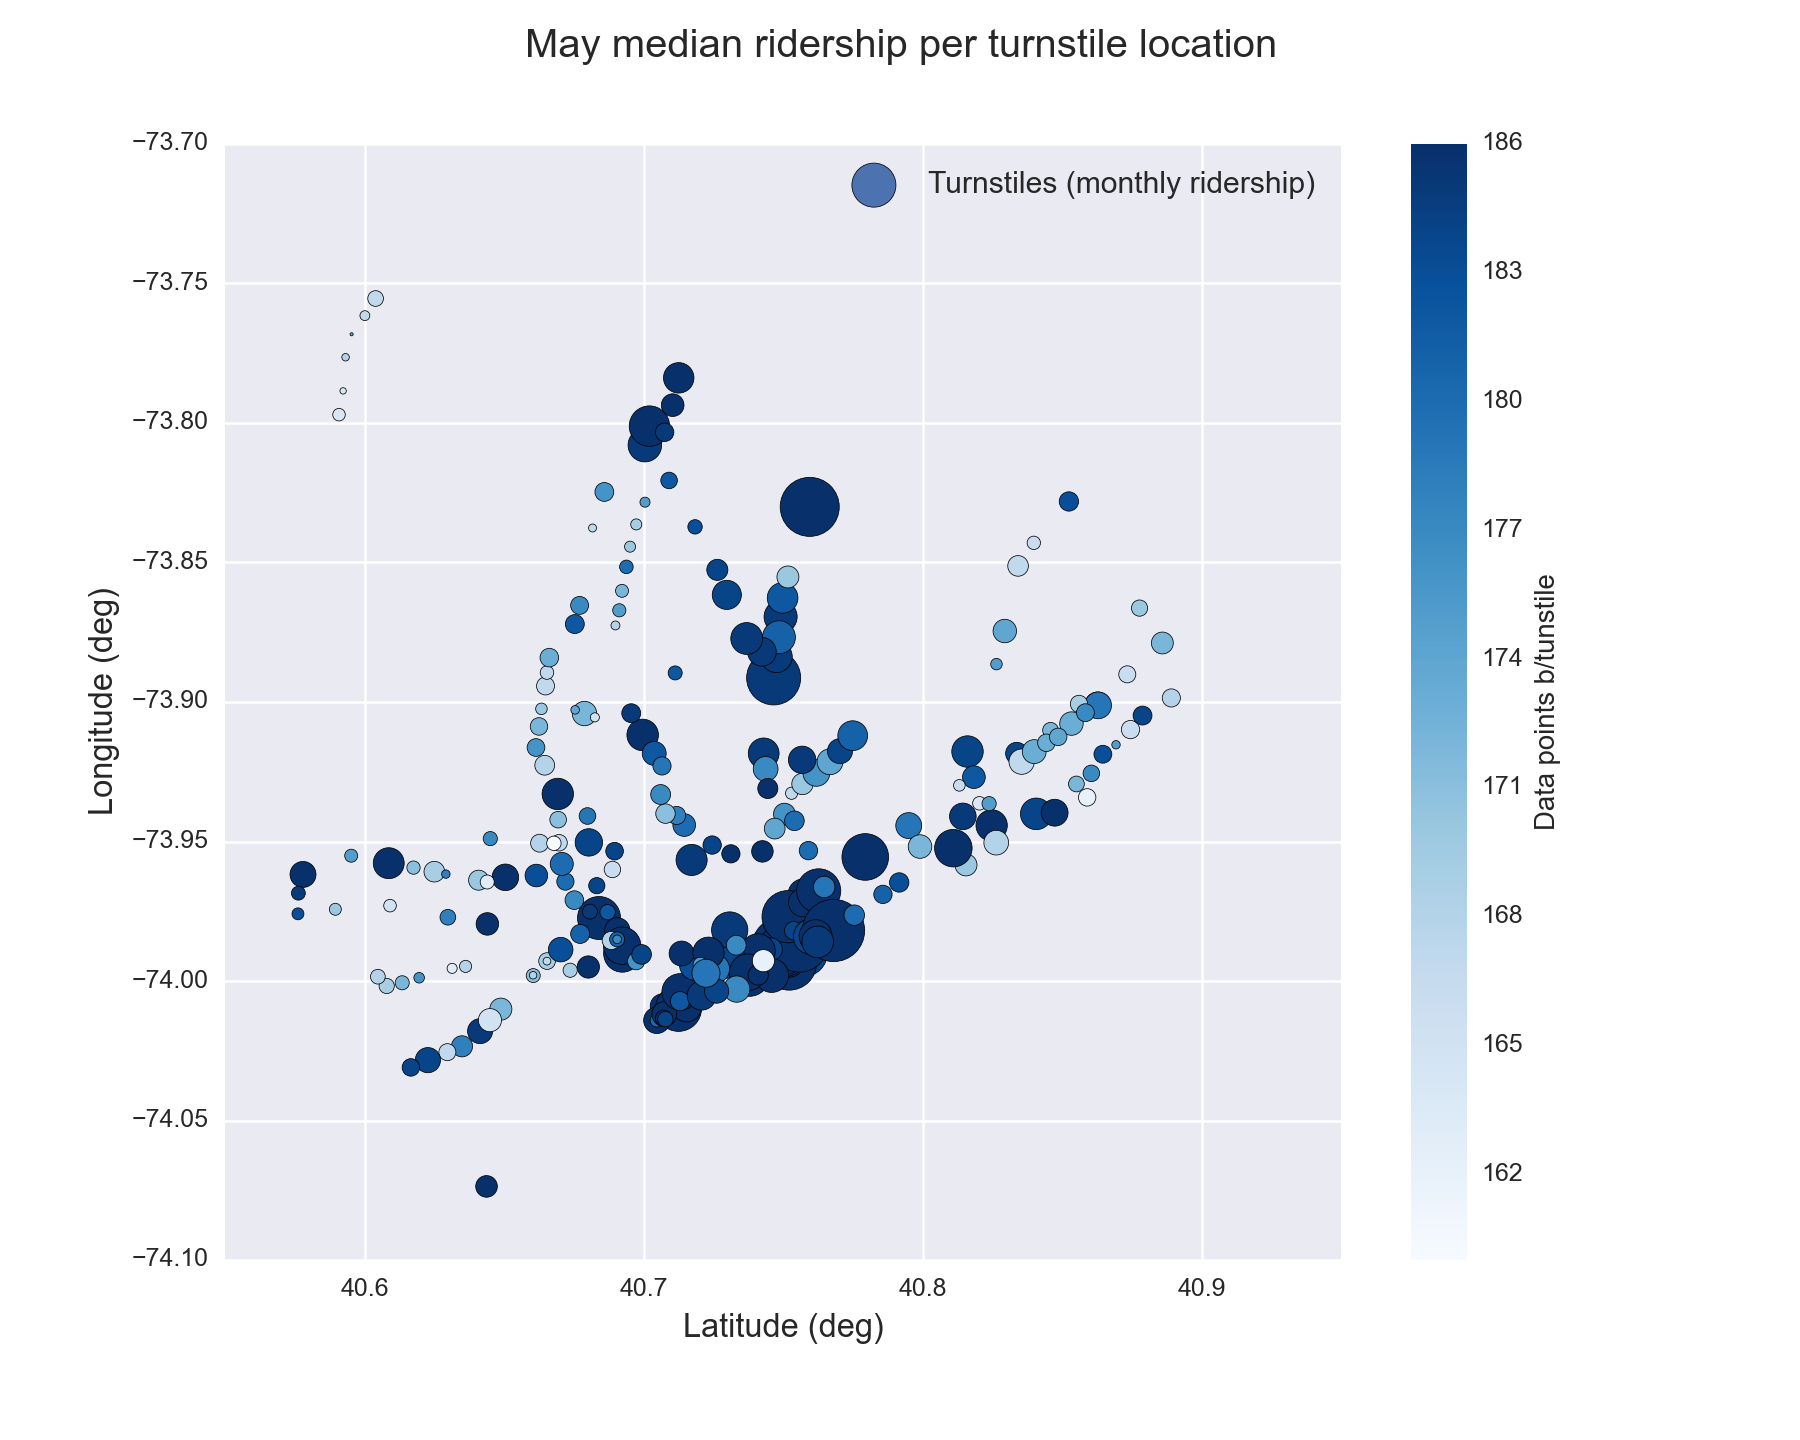
\includegraphics{medrider_loc.png}}
\caption{Turnstiles' locations within NYC, from the improved dataset.}\end{figure}

Besides the information provided by the NYC subway, the dataset also includes
weather information taken from several weather stations within the NYC area:
each turnstile, depending on the location in NYC, is merged with the weather
information of the closest weather station, thus providing temperatures, wind
speed, pressure, conditions, precipitations, etc.

The project focuses one main question: Does the weather conditions, specifically
precipitations, affect the NYC subway ridership? To answer this question we
will use exploratory tools, statistical tests and visualizations. Also, we will
try to fit a model to the data by choosing certain predicting features; will
the use of the precipitation variable improve the fit?


\section{Supporting Material}
\label{overview:supporting-material}
Within the project github repository you will also find an ipython notebook,
where most of the work done was recorded for reference.


\section{Some remarks about the datasets used}
\label{overview:some-remarks-about-the-datasets-used}
For this project we use the data set provided at Data Analyst Nanodegree's
portal for Project 1. The description of the variables can be found on...

However, after the exploratory and data analysis, we created another dataset by
further munging the improved dataset. The basic idea was to smooth out features that
might be caused by individual turnstiles or measurements. To do this, I
grouped the data by time stamp and aggregated the entries by hour by adding all
the entries. Also, the precipitation information for each
time stamp was included by means of two columns:
\begin{itemize}
\item {} 
\code{rain\_hour}: indicator (0 or 1) for precipitations for the particular date
date and time. It is 1 if for any of the stations the conditions were Rain,
Light Rain, Hard Rain or Light Drizzle at that moment.

\item {} 
\code{rain\_day}: indicator (0 or 1) for precipitations for the particular day
of the report. If at any station of our turnstiles the conditions reported
precipitations during the day the value is set to 1.

\end{itemize}


\chapter{Statistical Test}
\label{section1:statistical-test}\label{section1::doc}
In lecture 3 and its problem set, the following question was given \emph{Do rainy}
\emph{days affect the ridership of the NYC subway?} To answer this problem we began by
\begin{quote}

creating two samples from our data:
\end{quote}
\begin{itemize}
\item {} 
Sample A (\emph{No rain}) is a subgroup containing the entries where no rain was reported, using the
information of the \emph{rain} variable (\(rain = 0\))

\item {} 
Sample B (\emph{Rain}) is a subgroup with the entries where some precipitation was reported
by means of the \emph{rain} variable (\(rain = 1\))

\end{itemize}

By studying the distributions, using histograms, we were able to characterize
both data samples. We found out that both samples have a similar shape, clearly
not normal, and positively skewed ({\hyperref[section1:figure21]{\emph{figure 2.1}}}).
\begin{figure}[htbp]
\centering
\capstart

\scalebox{0.750000}{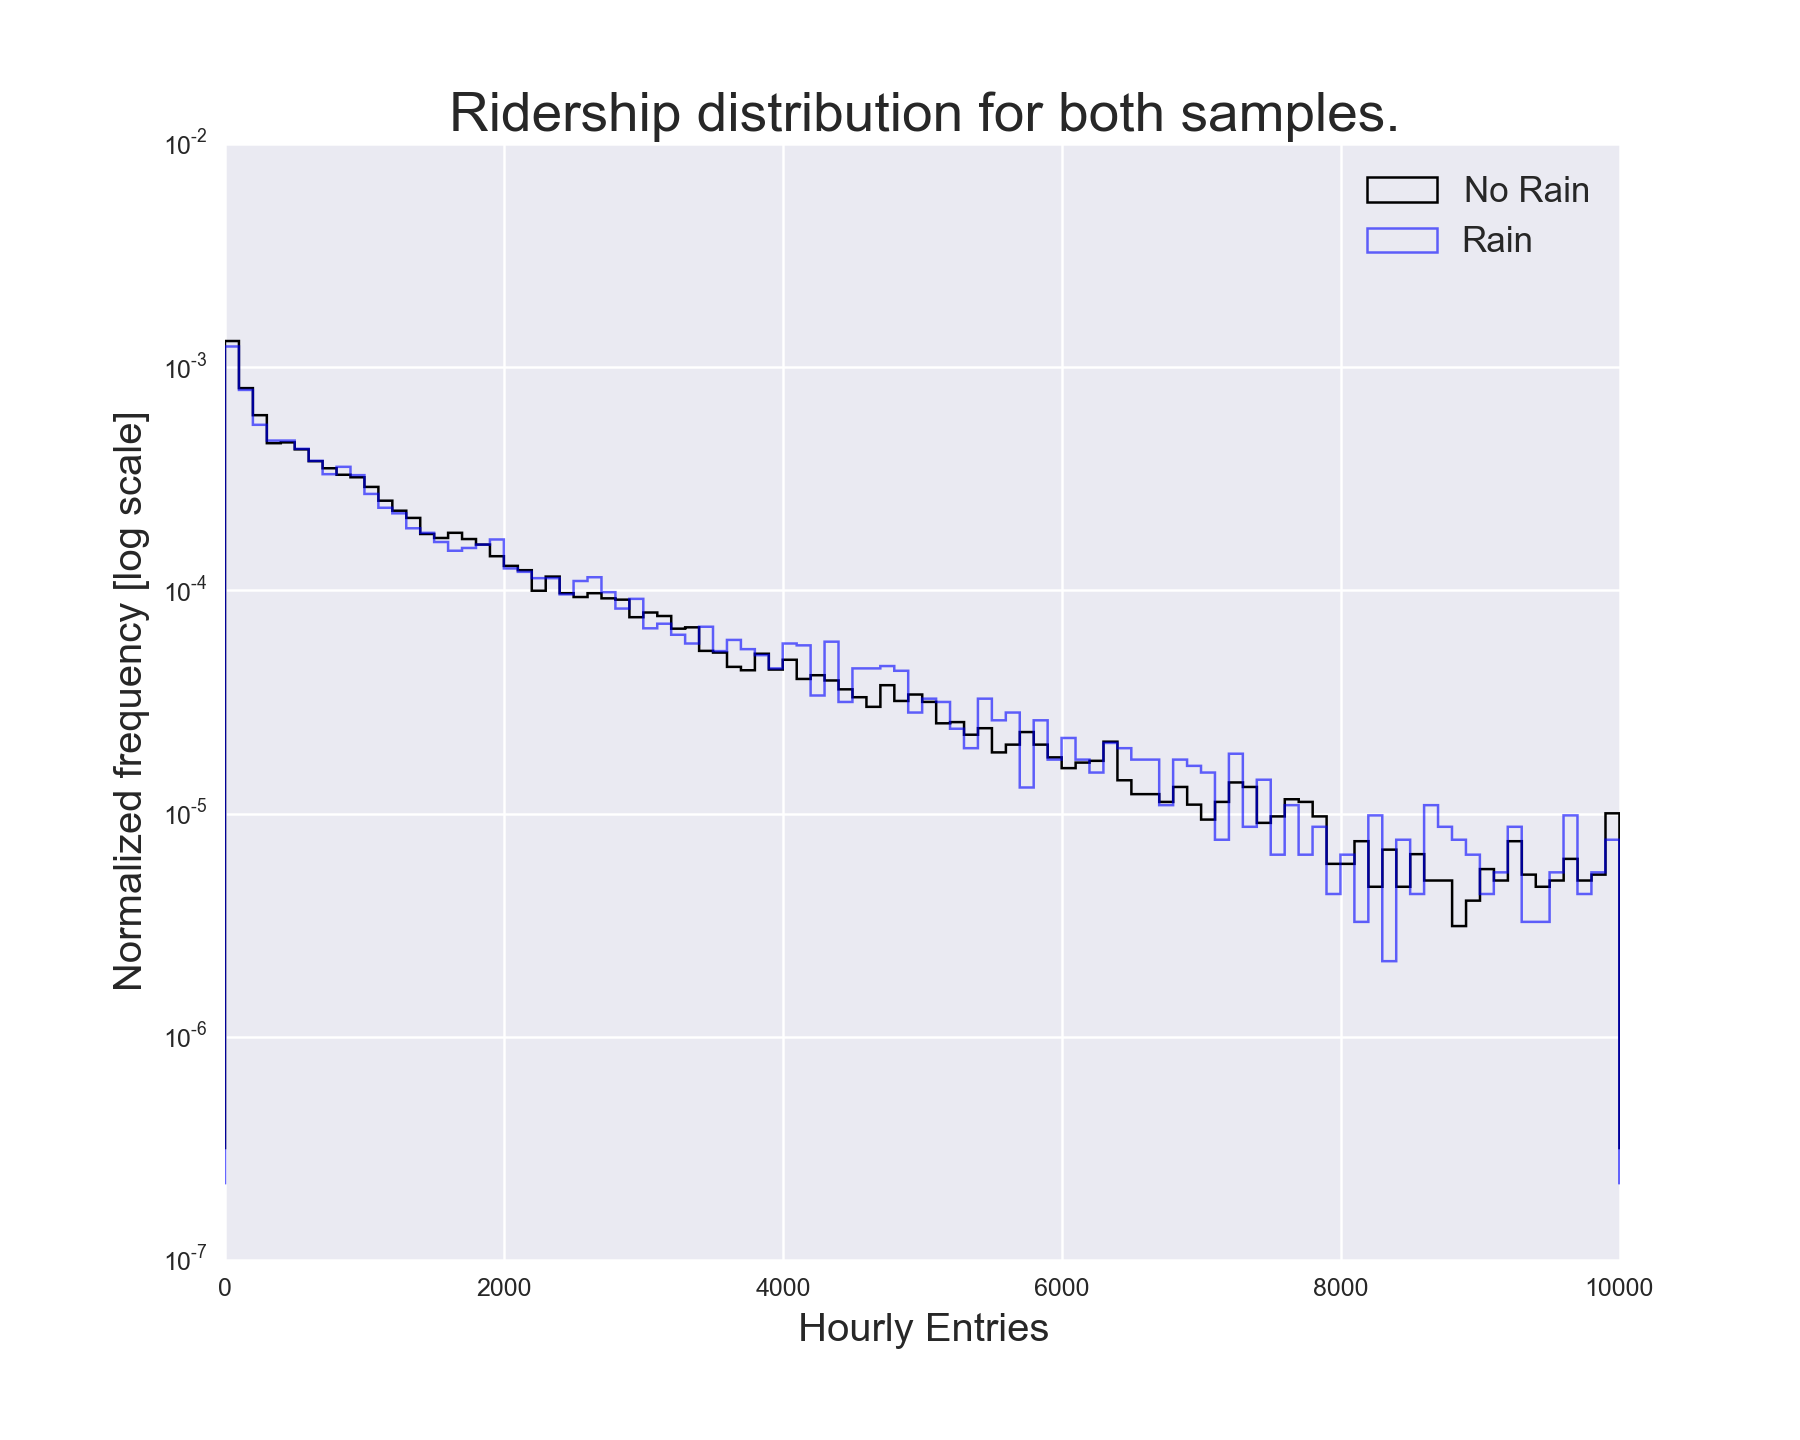
\includegraphics{samples_compared.png}}
\caption{Ridership distribution comparison between rainy and dry days.}{\small 
Please note the logarithmic scale on axis Y. It was used to allows us to study
the visualization with more detail.
}\label{section1:figure21}\end{figure}

Because of the non-normal distribution we decided to use the median as measure
of average for the samples:
\begin{itemize}
\item {} 
Sample A, days without precipitation, show a \textbf{median ridership of}
\textbf{901 passengers per hour.}

\item {} 
Sample B, rainy days, report a \textbf{median of 945 passengers per hour.}

\end{itemize}

To assess the significance of this result, that rain seems to increase ridership
in the NYC system by a small amount, we will use a non-parametric test.


\section{Statistical Test Used}
\label{section1:statistical-test-used}
The Mann Whitney U test is chosen to assess the statistical significance of this
result. The null hypothesis in our case is that both populations are equal, or
that there is no significant deviation on both populations medians (two-tailed
hypothesis).


\section{Justify the Statistical Test}
\label{section1:justify-the-statistical-test}
The Mann Whitney U test, or Wilcoxon rank-sum test, is chosen because of
characteristics of our samples: we can't use a parametric test because the
distributions do not seem to follow any particular and well known probability
distribution which we could use to make inferences that could directly report the
significance of any difference between both populations.

The U test is particularly powerful to assess the significance of the difference
between the median of two samples that have similar distributions. The assumptions
that our data samples must comply with are basically:
\begin{itemize}
\item {} 
All observations of both groups are independent

\item {} 
The responses are ordinal (so we can use the ranking algorithm of the U test).

\end{itemize}


\section{Results}
\label{section1:results}
We used the scipy implementation of the Mann Whitney U test
(scipy.stats.mannwhitneyu). The results from the test are:
\begin{itemize}
\item {} 
\(U = 150678745.0\)

\item {} 
\(p = 1.91 \cdot 10^{-6}\)

\end{itemize}

But the user should be aware that scipy reports p-value for a one-tailed
hypothesis, so we multiply by 2 to get the significance for our hypothesis:
\begin{itemize}
\item {} 
\(p = 3.82 \cdot 10^{-6}\)

\end{itemize}


\section{Interpretation and discussion}
\label{section1:interpretation-and-discussion}
The interpretation, given the result from the U test, is that the the ridership
is not the same for rainy days than non-rainy days, with a significance higher
than 95\% (p \textless{} 0.05). Furthermore, from the descriptive statistics of our samples
we can conclude that the ridership tends to be higher in rainy days.

However we have limited ourselves here to follow the procedure suggested by the
lectures, assuming that observations of both groups are independent and there
no other factors that might wrongly induce this result. Even when the data sample
we use for the project has been through a more complete wrangling, there are
still some issues that might affect the results:
\begin{itemize}
\item {} 
There is missing data for several turnstiles. From the original sample of 240
turnstiles, only 52 have complete data for May; also, as discussed on the forums,
some precipitation data is missing from some weather stations.

\item {} 
We are using the variable \emph{rain} to create our samples: this variable
indicates if the conditions at anytime of the day at a
particular turnstile were rainy. Is it the appropriate variable to use to
build the subgroups?

\item {} 
There is one day which was a holiday (Monday 30th), should the data from this
day be discarded?

\end{itemize}

Let's look with more detail at some these problems.


\subsection{Missing data and precipitation distribution}
\label{section1:missing-data-and-precipitation-distribution}\begin{figure}[htbp]
\centering
\capstart

\scalebox{0.750000}{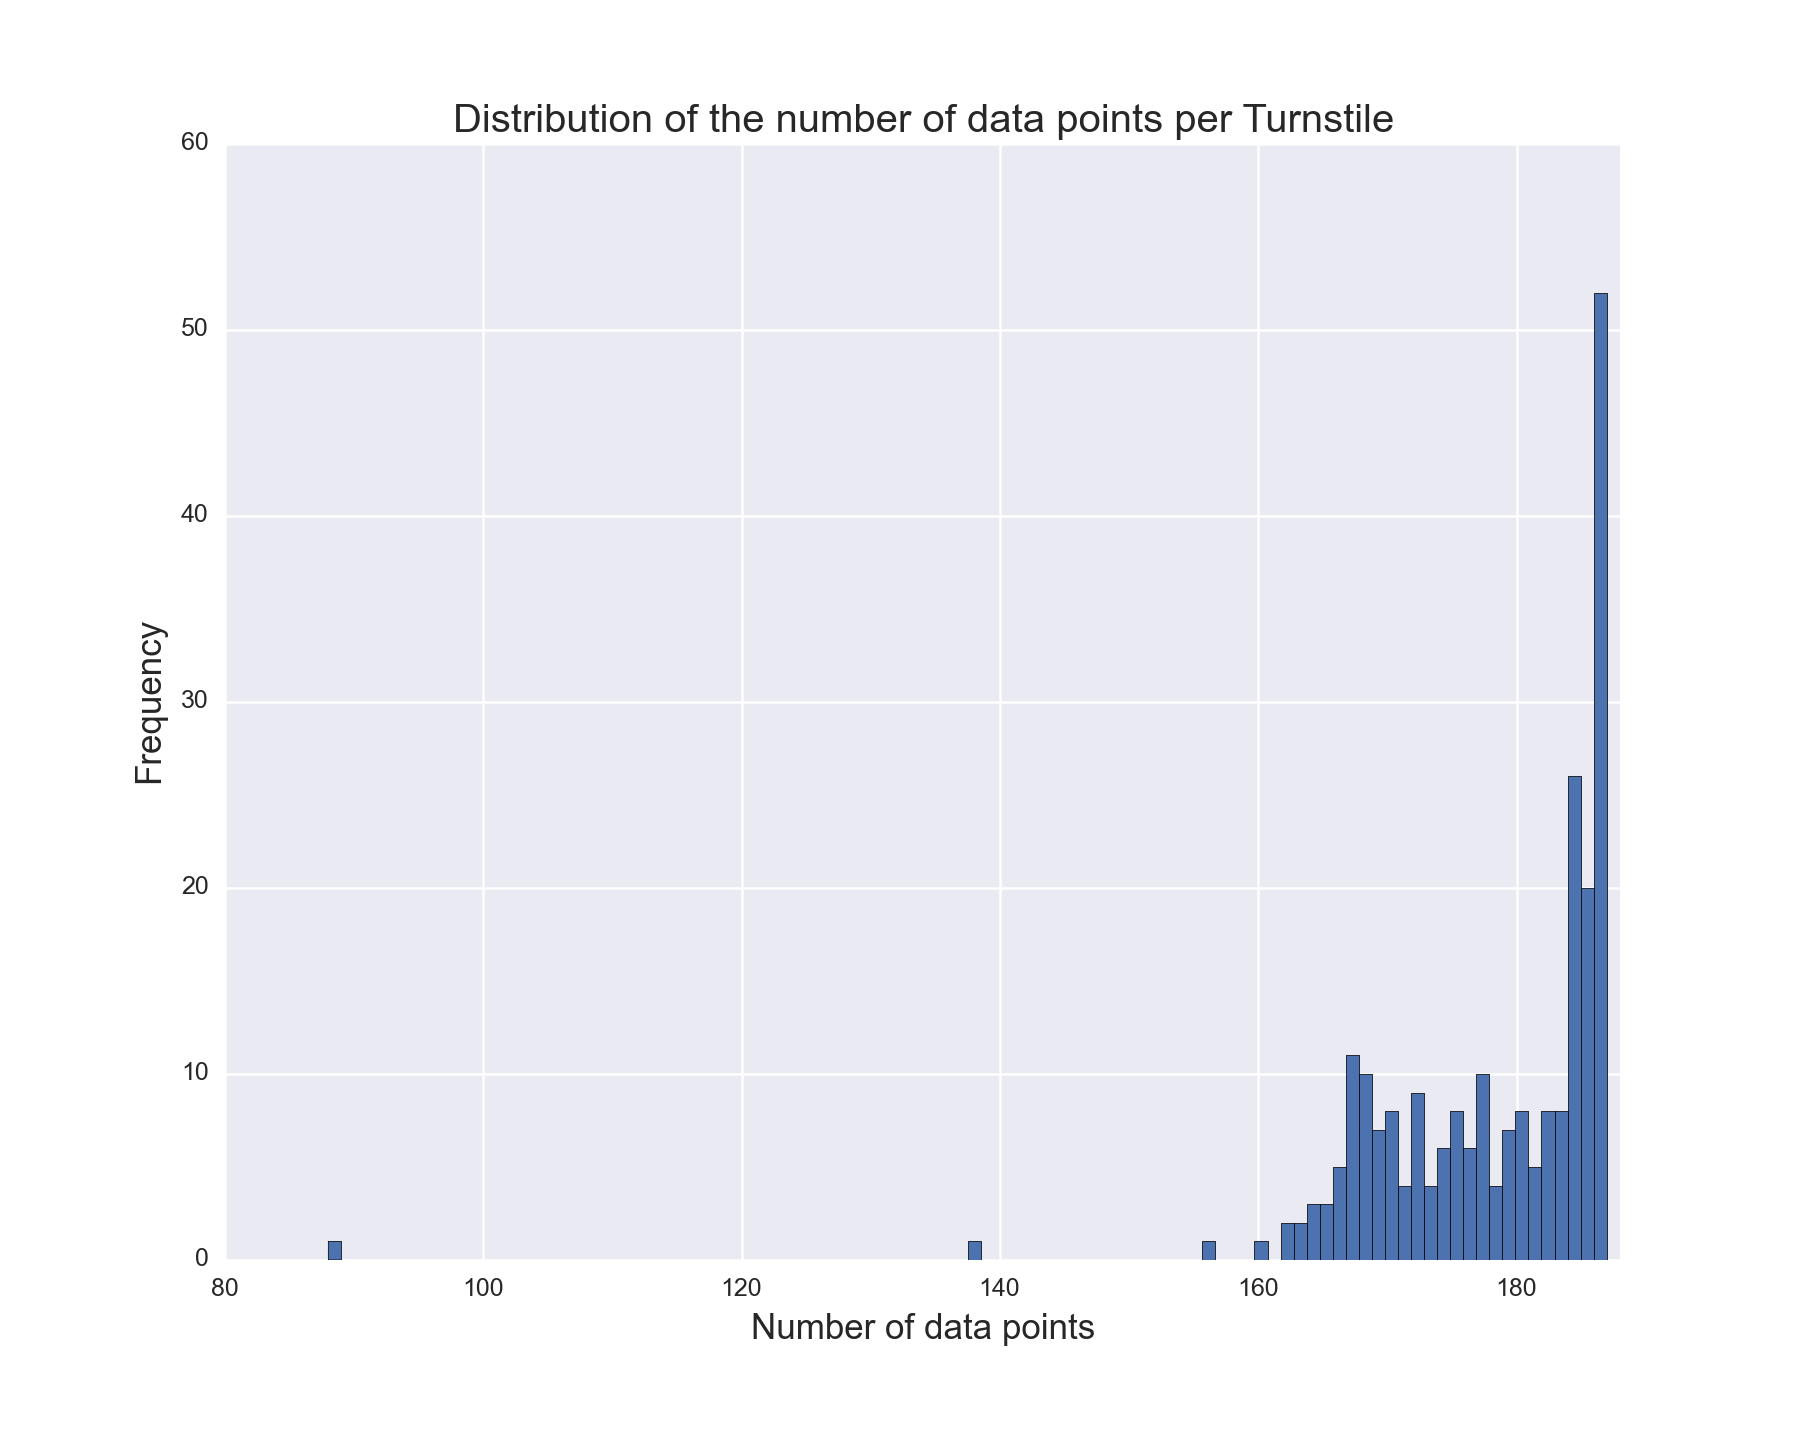
\includegraphics{dataentries.png}}
\caption{Number of data points (measurements) by turnstile on project's improved
dataset.}\label{section1:figure22}\end{figure}

{\hyperref[section1:figure22]{\emph{Figure 2.2}}} shows some turnstiles have missing data for the
month of May; with 31 days and 6 daily reports it is expected that a complete
monitored turnstile should have 186 measurements. This is the case for 52 turnstiles,
but 185 turnstiles have a number of measurements between 160 and 185. 3 turnstiles
had less than 160 entries, and after inspections they have been removed because
of the huge amount of missing data or time stamps reporting 0 entries. Of the 185
turnstiles with incomplete data, there was one case where at all time stamps the
number of entries was 0, which was also removed as it does not add any information
to our analysis (even when in other cases it could give further information).

The problem with the missing data is that, for some not clear explanation we
could provide, affects more the suburb stations turnstiles than the ones in downtown
areas. And suburb stations tend also to show lower number of hourly entries, i.e, a
lower ridership, than downtown turnstiles. This effect can be seen in
{\hyperref[section1:figure23]{\emph{Figure 2.3}}}.
\begin{figure}[htbp]
\centering
\capstart

\scalebox{0.750000}{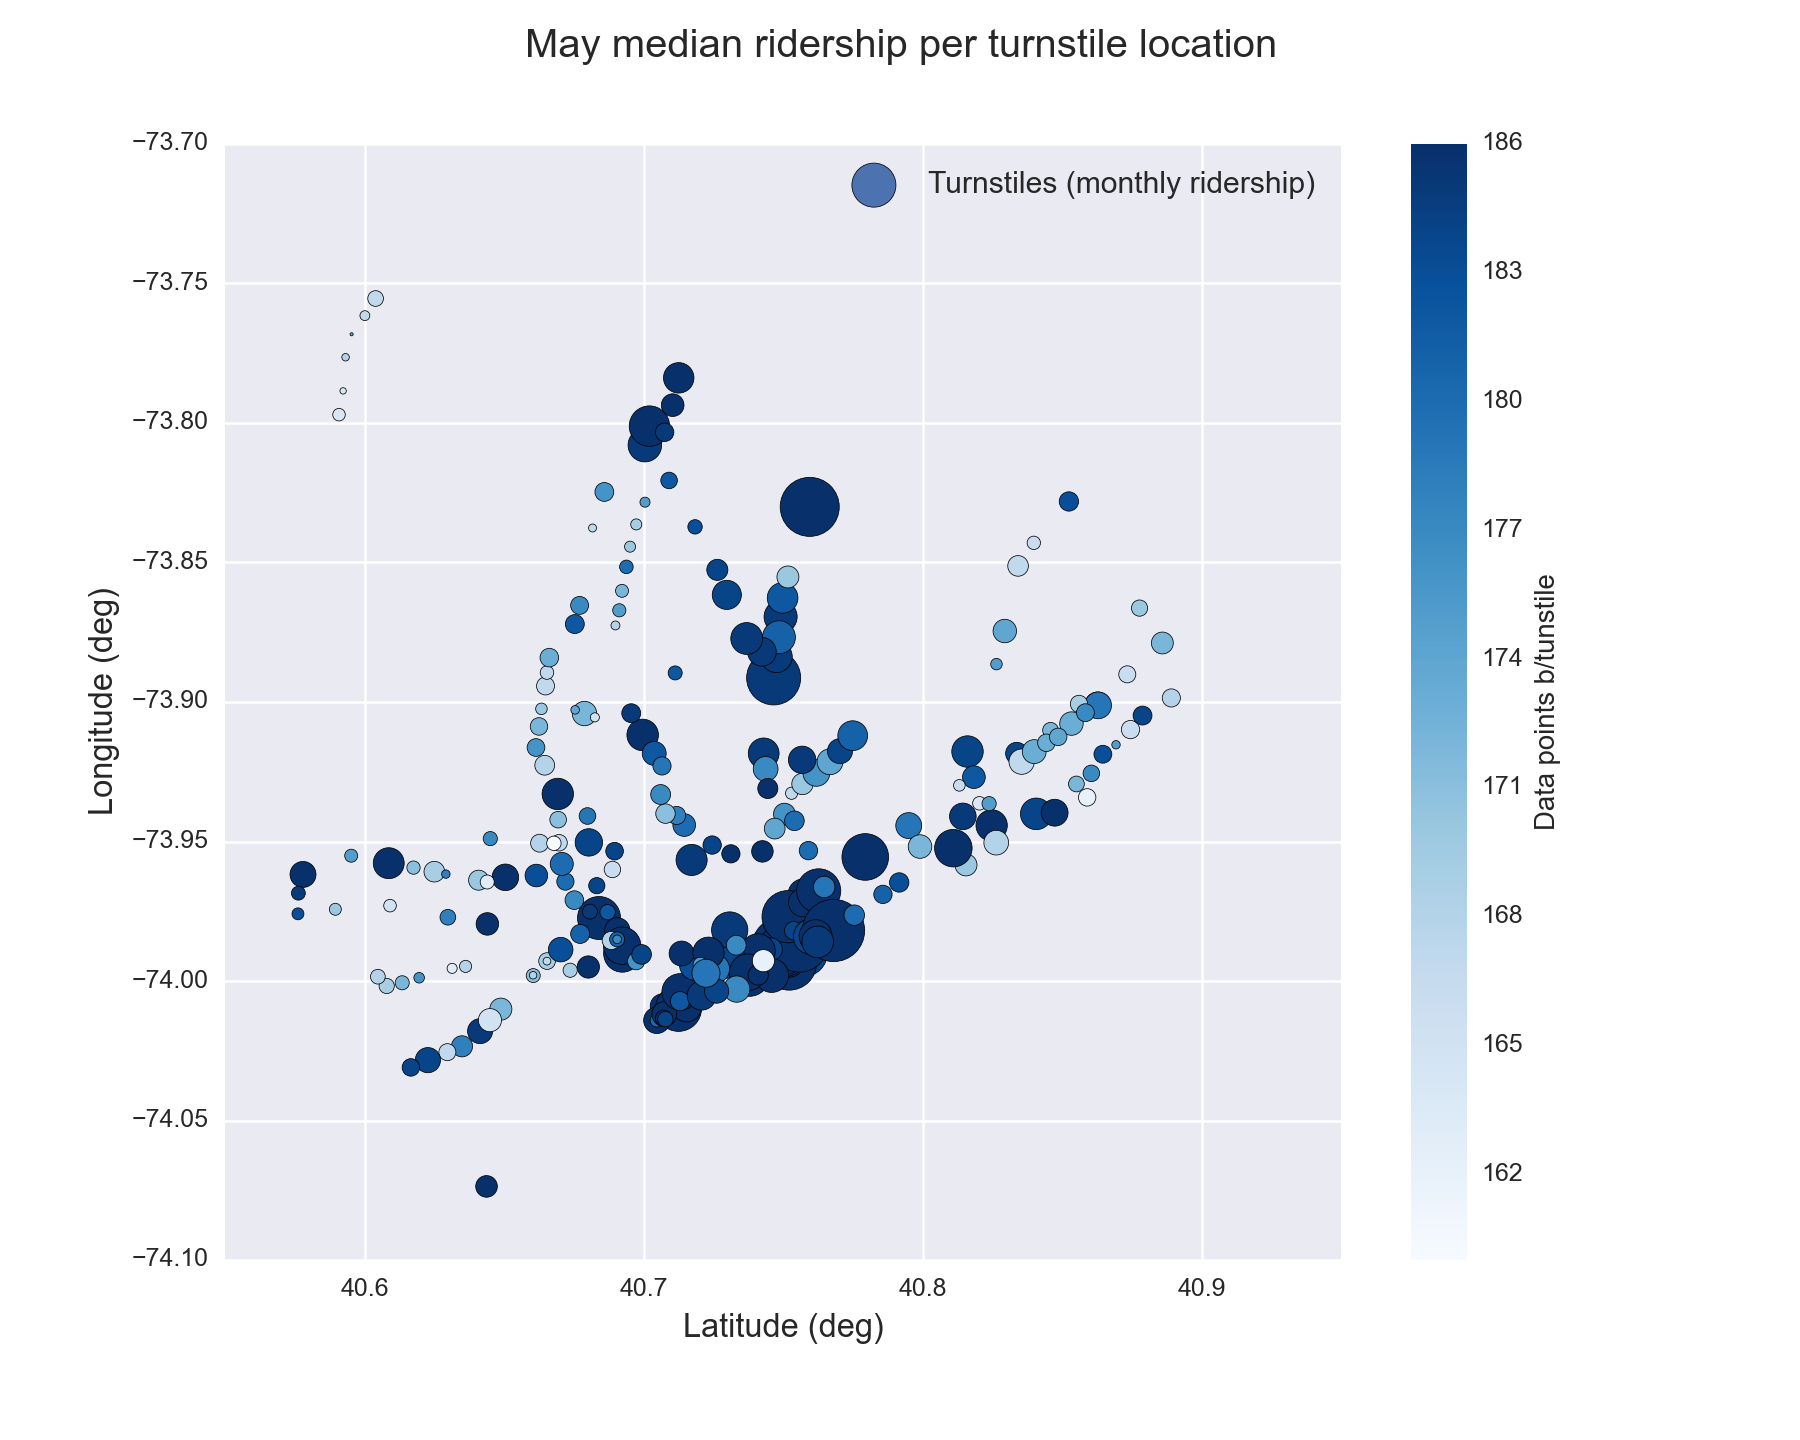
\includegraphics{medrider_loc.png}}
\caption{Turnstiles monthly median ridership, location and number of data points}{\small 
The figure shows the distribution of the turnstiles within NYC which are in
our dataset. The size is proportional to the monthly median ridership (entries
by hour) while the color indicates the data completeness of each turnstile: whiter
colors indicate locations with more missing data.
}\label{section1:figure23}\end{figure}

We wonder, as the reader also may, if this missing data could affect in anyway
our previous study. We are not completely sure, but we think that given the way
we performed our analysis it could happen that the results were affected: the downtown
station data, which also correspond to the group of stations with higher ridership,
is contributing to increase the median ``entries by hour'' that we calculated, as they are
located in the higher values side of the ridership distribution. What happens if
the stations in this locations are also the ones that tend to have more rainy days?
We didn't believe this was the case, but just to be sure we created the
plot shown in {\hyperref[section1:figure24]{\emph{Figure 2.4}}}.
\begin{figure}[htbp]
\centering
\capstart

\scalebox{0.750000}{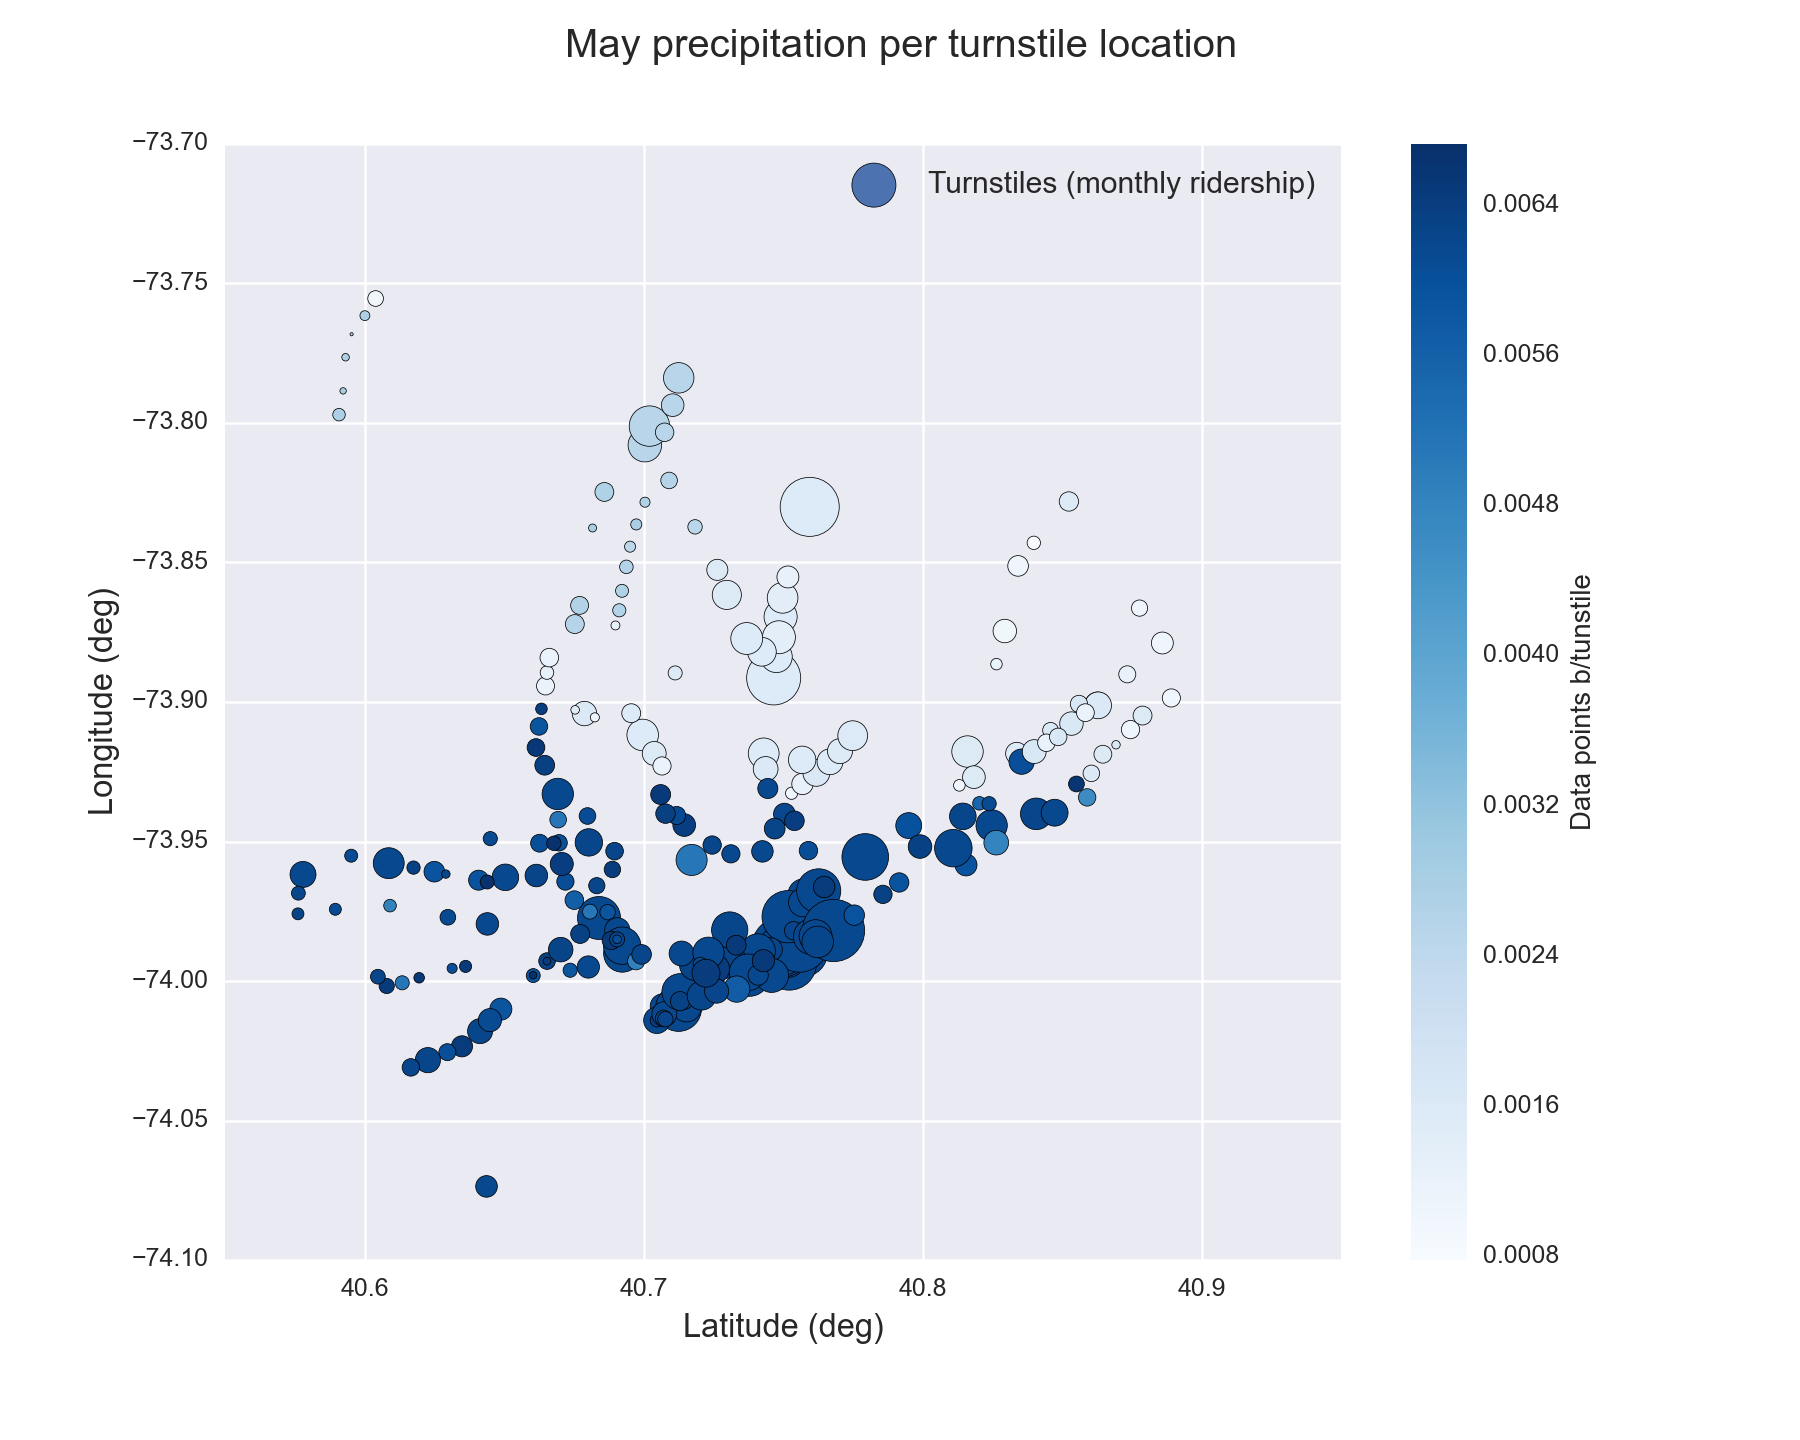
\includegraphics{medprecip_loc.png}}
\caption{Turnstiles monthly median ridership, location and mean precipitation.}{\small 
The figure shows the geographical distribution of the NYC turnstiles in the
project's improved dataset. Size is proportional to the monthly median ridership
and color represent the month's mean precipitation per turnstile. The figure
shows that precipitations are higher in southern (and downtown) NYC.
}\label{section1:figure24}\end{figure}

The figure shows that the precipitation is higher in the northern NYC, which is
also the location of the most busy turnstiles: the median ridership of stations with
higher precipitation (\textgreater{} 0.004 inches) is 1116 entries by hour, while the stations
with lower precipitation (\textless{}= 0.004 inches) is 832 entries by hour. Also the stations
with higher precipitation report on average 7 rainy days while the lower precipitation
turnstiles only report 6.


\subsection{The use of the \emph{rain} variable}
\label{section1:the-use-of-the-rain-variable}
The \emph{rain} indicator in the improved data set reports if whether any precipitation
happened at the turnstile location during the day. Because some of the
precipitation data was missing in the weather tables, the conditions
reported in the \emph{conds} variable was used to create the \emph{rain} column (as
mentioned in the forums): if at anytime during a day the condition reported at
a turnstile location was one of the following the \emph{rain} indicator was set to one:
`Rain', `Light Rain', `Heavy Rain' or `Light Drizzle'. This explains why for 94
entries reporting \emph{rain} equal to 1, the \emph{meanprecipi} variable (mean precipitation
for the day at the location) was 0. Also, as shown before, this indicator is different
for each turnstile depending on the closest weather station report. Thus, we
find out that 216 turnstiles report 7 days of rain, 19 turnstiles report 6 rainy
days, and 2 report 5 rainy days. Adding this analysis with the one in the previous
subsection, we have to be aware that the samples might not be completely independent
as previously thought.

Also, there is another important problem derived from the use of \emph{rain}
variable that we hope to make clear with the plot shown on
{\hyperref[section1:figure25]{\emph{Figure 2.5}}}.
\begin{figure}[htbp]
\centering
\capstart

\scalebox{1.000000}{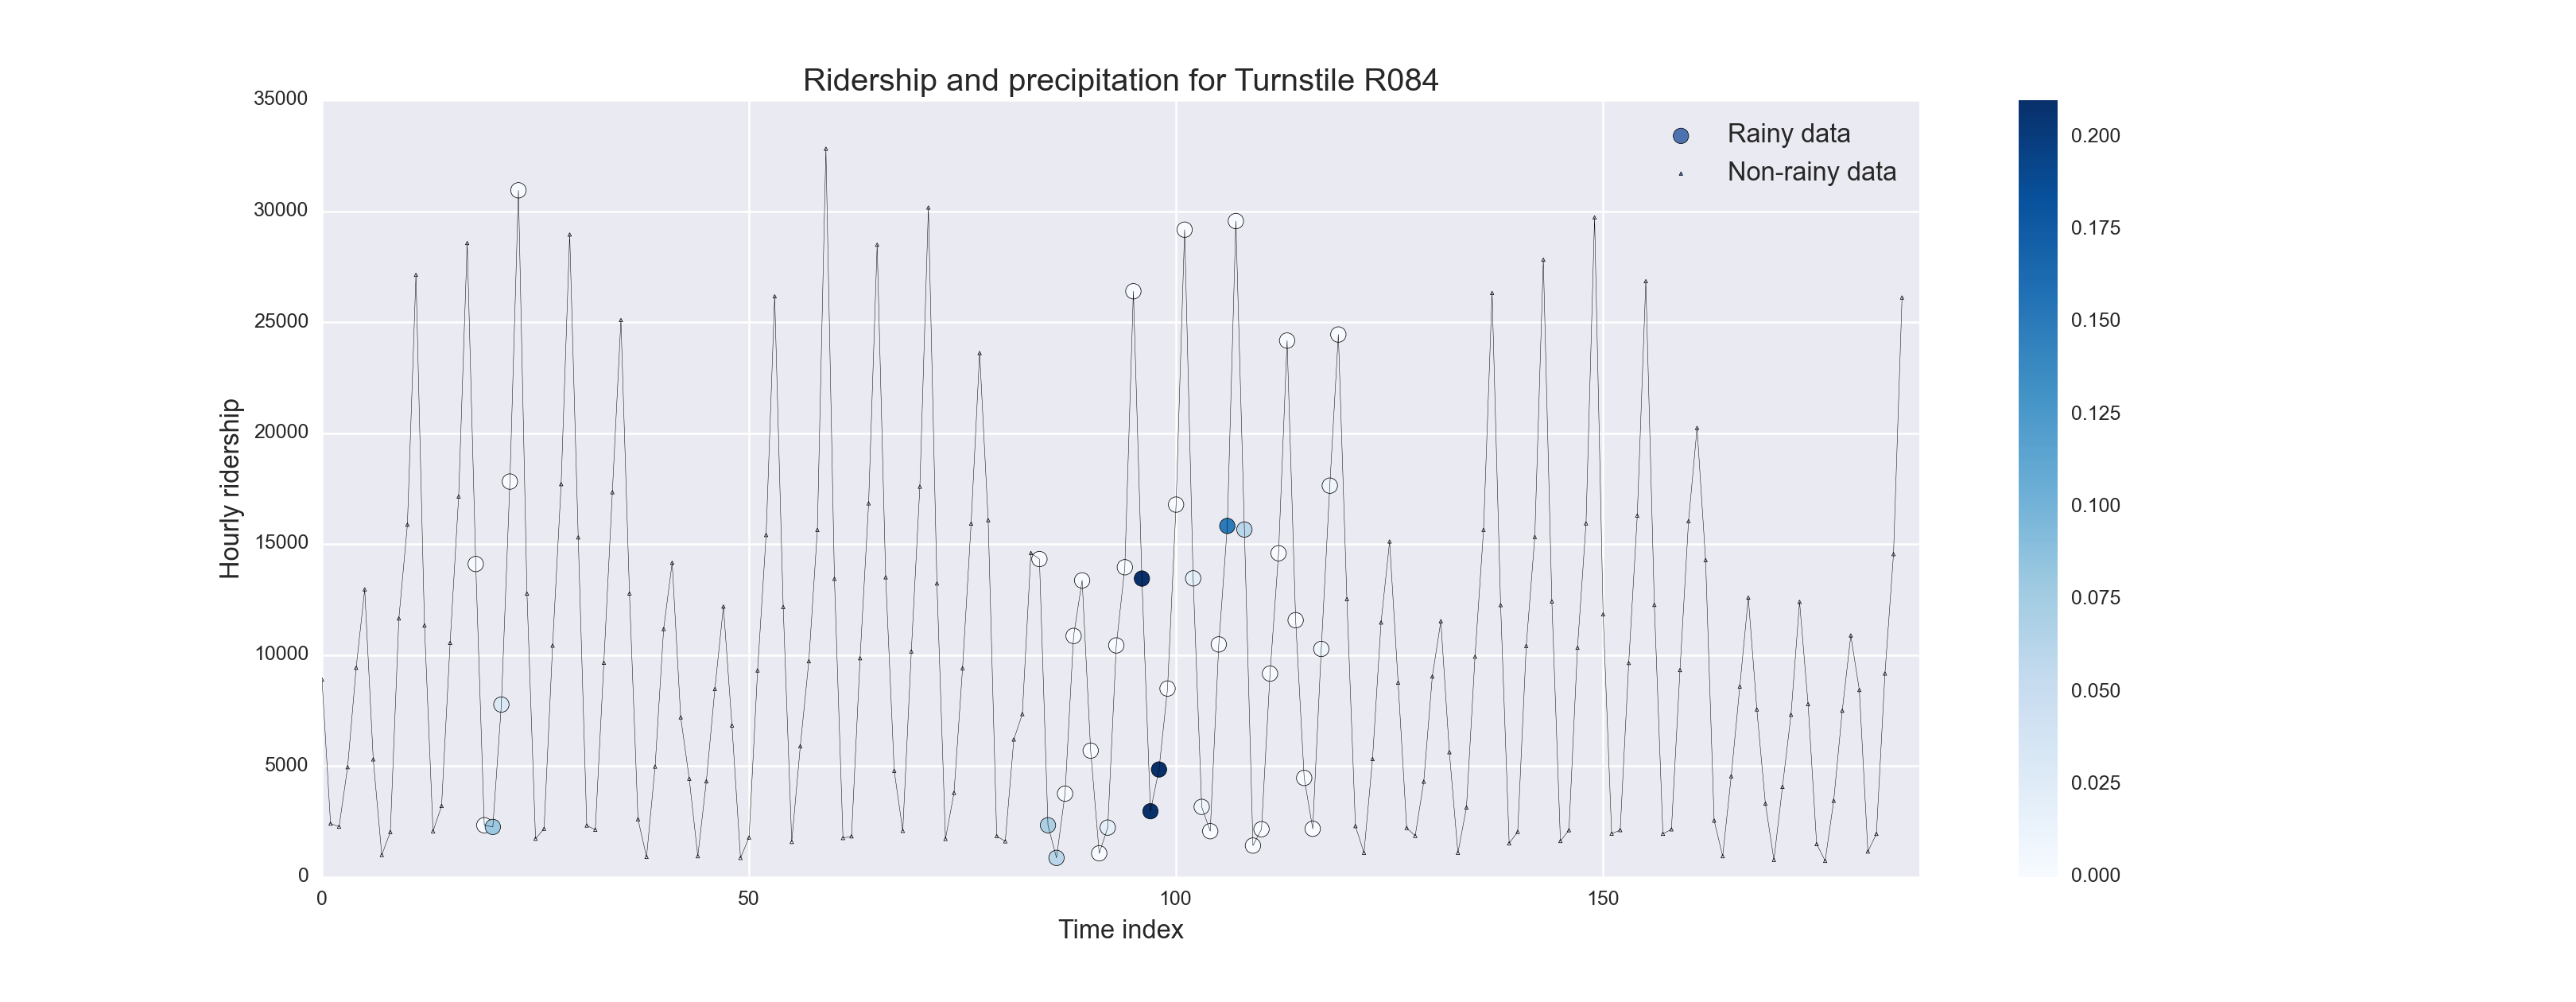
\includegraphics{r084.png}}
\caption{Ridership, precipitation and rain indicator for turnstile 084.}{\small 
The figure show the ridership evolution in May, in terms of entries per hour,
for turnstile 084, which is on one of the must busy stations in NYC subway.
There is one point every four hours for the month of May, and the symbols indicate
whether the day was rainy (big circles) or not rainy (small triangles). Also,
the precipitation amount in inches for the rainy days is shown by means of the
color bar in the right, with darker blue colors indication more precipitation.
}\label{section1:figure25}\end{figure}

The problem we see on using the \emph{rain} variable as and indicator of rainy conditions
for a turnstile is that a whole day is tagged as rainy even when only rain at one
time during the day. Furthermore, it can happen, as it can clearly be seen on the figure,
that the rain happened in one of the less busy hours of the day, but still the whole
day data will be tagged as rainy: this will clearly affect the results of our
previous analysis.


\subsection{Smoothing the data and answering the question again}
\label{section1:smoothing-the-data-and-answering-the-question-again}
In order to smooth out the previously mentioned effects we created a new data
set from where two samples will be created later. For this dataset we grouped
all individual turnstiles data by time stamp, aggregating the ridership
(\emph{ENTRIESn\_hourly}) using the \emph{sum} function. In this way we have a set that
represent the behavior of the whole NYC subway as one system, instead of
individual turnstiles, reporting the total ridership at each time stamp. For each
time stamp a variable called \emph{rain\_day} was created, which is 1 if in any
turnstile during a day within the whole NYC subway network some precipitation
was reported, or 0 otherwise. Also, the data from May 30th is removed, since it
changes the statistic for the mondays. We will now redo the analysis using this
dataset, and in this way try to answer the original question: \emph{Does the NYC subway}
\emph{ridership changes with the precipitation conditions?}
\begin{itemize}
\item {} 
Sample A is the subgroup of all the data coming from non rainy days (\emph{rain == 0}).

\item {} 
Sample B is the subgroup of the data in rainy days (\emph{rain == 1}).

\end{itemize}

The ridership distribution of both samples are again similar in shape, but they are not
longer continuous, as show in {\hyperref[section1:figure26]{\emph{Figure 2.6}}}. We will use again the median
to report the average of each sample, and the Mann Whitney U test to assess the significance
of any difference we might found.
\begin{figure}[htbp]
\centering
\capstart

\scalebox{0.750000}{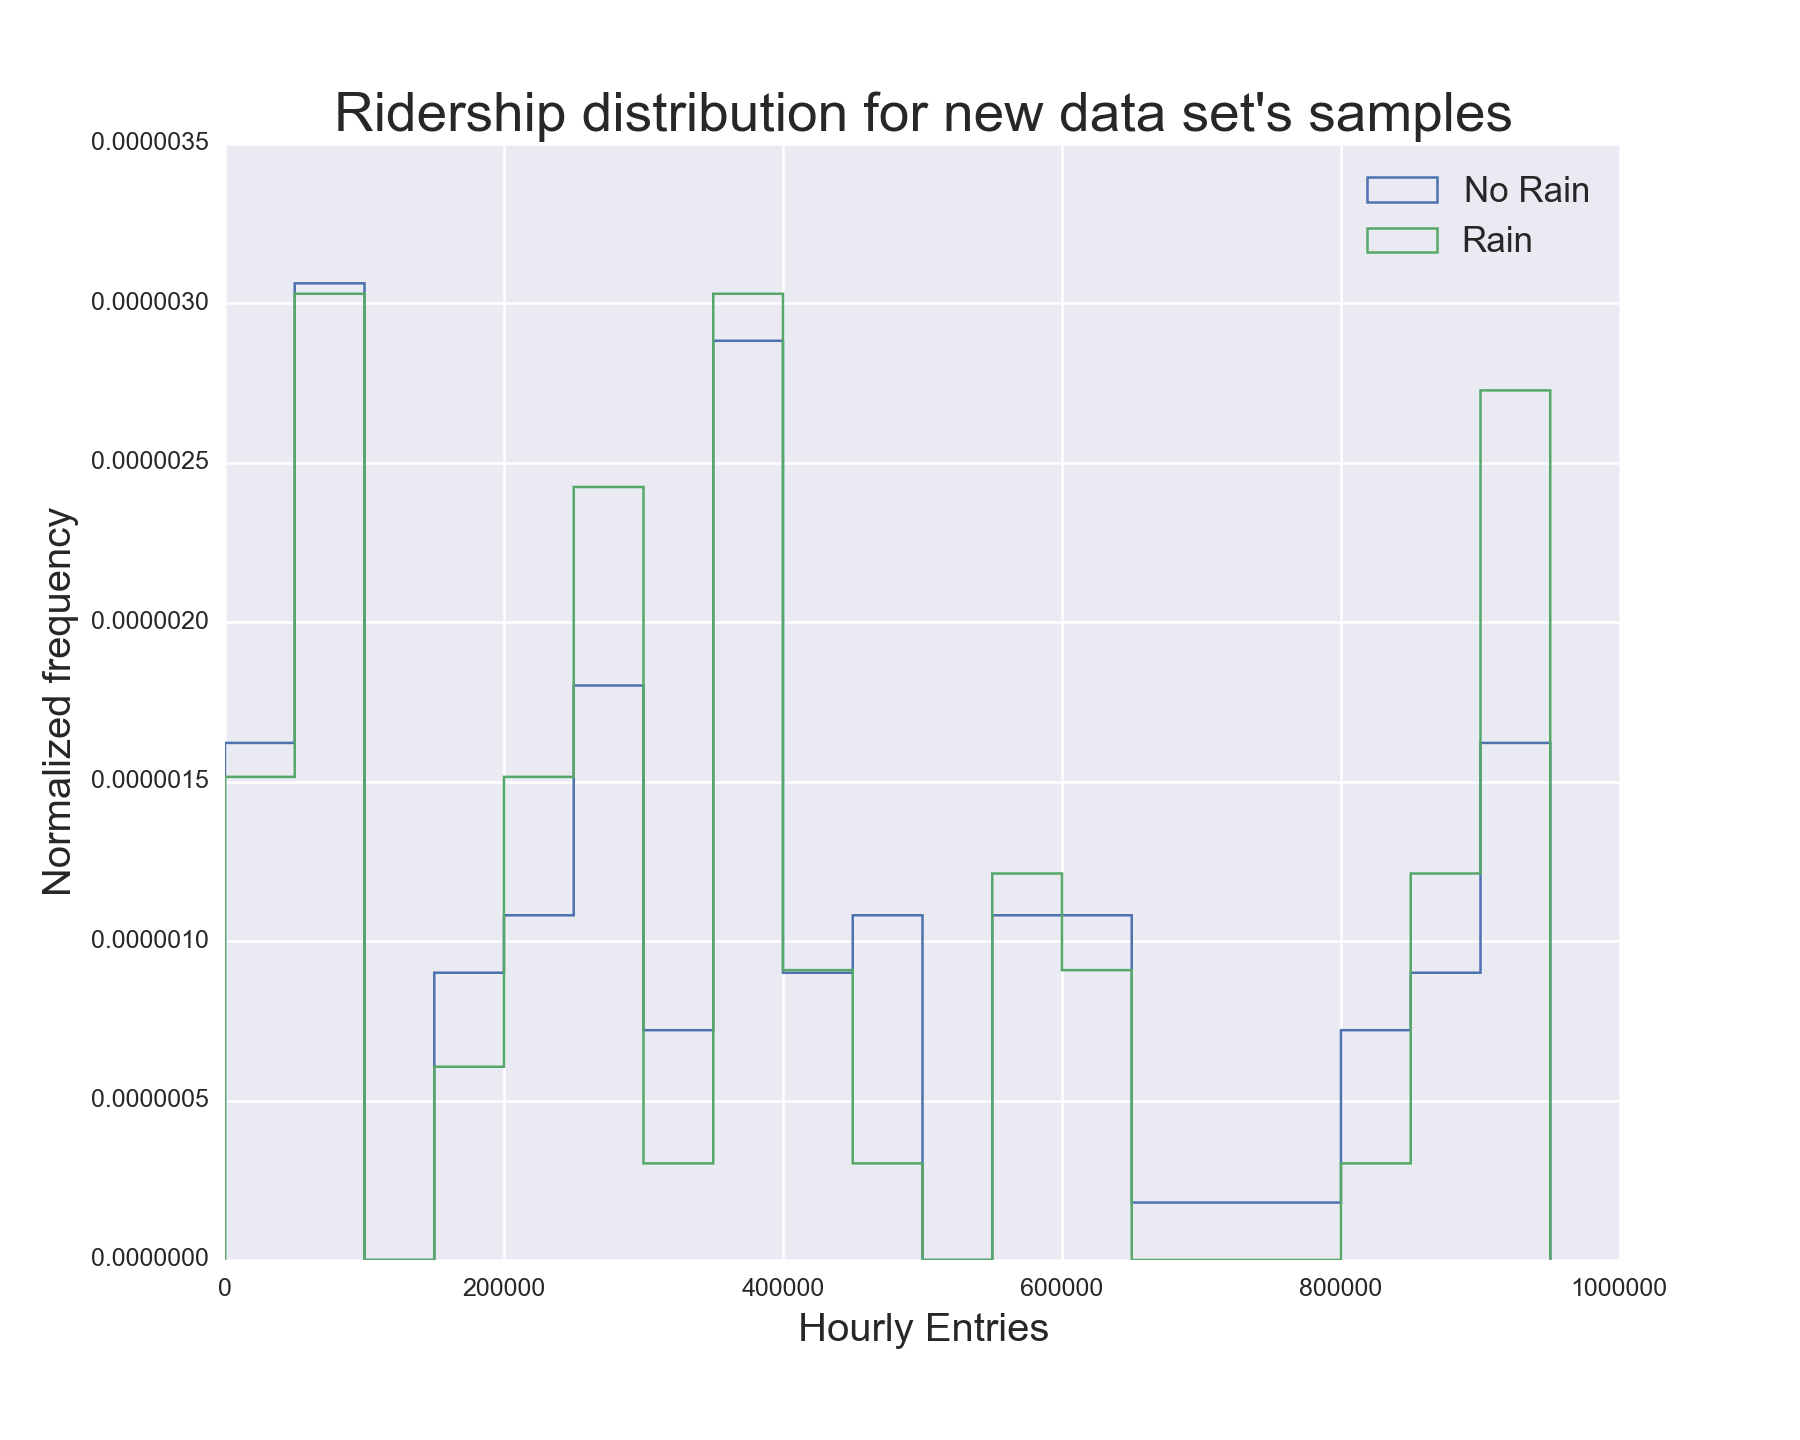
\includegraphics{samples2_compared.png}}
\caption{Ridership distribution comparison between rainy and dry days for the new samples
taken from the aggregated data.}\label{section1:figure26}\end{figure}

The ridership in non-rainy days has a median of 370535 entries per hour, while for rainy
days the median is 363124. However the results from the U test are now different:
\begin{itemize}
\item {} 
U statistic: 3477.0

\item {} 
p-value (2-tailed hypothesis): 0.71

\end{itemize}

So the difference in the medians are not significant now, and we can't conclude that
there is any meaningful difference in the ridership as a function of the precipitation
conditions.


\chapter{Linear Regression}
\label{section2:linear-regression}\label{section2::doc}
The second part of this work deals with the use of tools related to machine
learning: can we use the data to create models that will allows us to predict
the ridership?

Problem Set 3 of the class has as one of the main goals the use of a linear
regression model that could help us to predict the ridership in the NYC subway.
We were asked to implement one of the algorithms that calculates the coefficients
of a multiple linear regression model: gradient descent. The selection of the
features, and thus the number of coefficients to fit, was left as an exercise
for the student.

After implementing the linear regression model, and study its strengths and
shortcomings, we used another algorithm to find the coefficients of the linear
regression model: OLS, or ordinary least squares.

Finally, a third method was used, also based on a linear regression algorithm,
but this time the model used higher order polynomials to learn from the data,
in an effort to fit the non-linearity of it.


\section{Linear regression algorithm(s)}
\label{section2:linear-regression-algorithm-s}

\subsection{Gradient descent}
\label{section2:gradient-descent}
The code used to implement the gradient descent algorithm to find the linear
regression coefficient can be checked on the python file available at the
github repository associated to this work, and on the submissions to the
\emph{Introduction to Data Science} class (problem set 3).


\subsection{Ordinary Least Squares (with statsmodels)}
\label{section2:ordinary-least-squares-with-statsmodels}
Selecting the same features as in the Gradient Descent exercise, we calculated
the coefficients of the linear model by using the OLS implementation of the
statsmodels python library.


\subsection{Polynomial features with Ridge linear regression}
\label{section2:polynomial-features-with-ridge-linear-regression}
After analysing the results from the previous regressions, and for reasons that
will be clear after the description of their results, we went a little further
and we used a polynomial transformation of the selected features, and another
linear regression algorithm, the Ridge regression, was used to model the data
and predict ridership. The model used and results will be shown in the
interpretation section.


\section{Models and features used}
\label{section2:models-and-features-used}
The selection of the features to use and how to use them in the model was not
a linear process, but an iterative work based on exploratory statistics, residuals
analysis and study of the models obtained to predict the ridership. If fact,
for the problem set 3 in the class we used a different set of variables as
predictors (specifically \emph{day\_week} instead of \emph{weekday}).

Also, because of these iterative analysis we decided to also give a try to a
third method to model the data, which was the use of polynomial features.

The multiple regression model used for the first two methods can be written as:
\phantomsection\label{section2:multreg-mod}\phantomsection\label{section2:equation-multreg_mod}\begin{gather}
\begin{split}\hat y = \theta_0 + \theta_1 x_1 + theta_2 x_2 + ... + \theta_k x_k\end{split}\label{section2-multreg_mod}
\end{gather}
where \(\hat y\) is the predicted variable, \(x_i\) are the predictors
(features) and \(\theta_i\) are the coefficients or parameters that we are
looking for using either the gradient descent or the OLS algorithms.

For our work, we decided to use the following predictors:
\begin{itemize}
\item {} 
\emph{UNIT}: turnstile unique identification. The use of the identification
of each turnstile starts from the realization that the turnstiles have different
ridership volumes for the same time periods, as it can be readily seen by
comparing ridership averages. However this is a non-numerical categorical
variable, so it was required to transform this variable to numerical format
by using dummy variables. This steps adds at once \emph{n} extra features or predictors,
one for each turnstile in our data, which adds a lot of computing work to the
algorithm.

\item {} 
\emph{hour}: numerical variable that indicates the hour of the day when the ridership
was reported for each turnstile. This variable takes values that can be continuous
between 0 and 24; it adds one coefficient to calculate. {\hyperref[section2:figure31]{\emph{Figure 3.1}}}
shows the relation of the ridership values with hour the day.

\end{itemize}
\begin{figure}[htbp]
\centering
\capstart

\scalebox{0.800000}{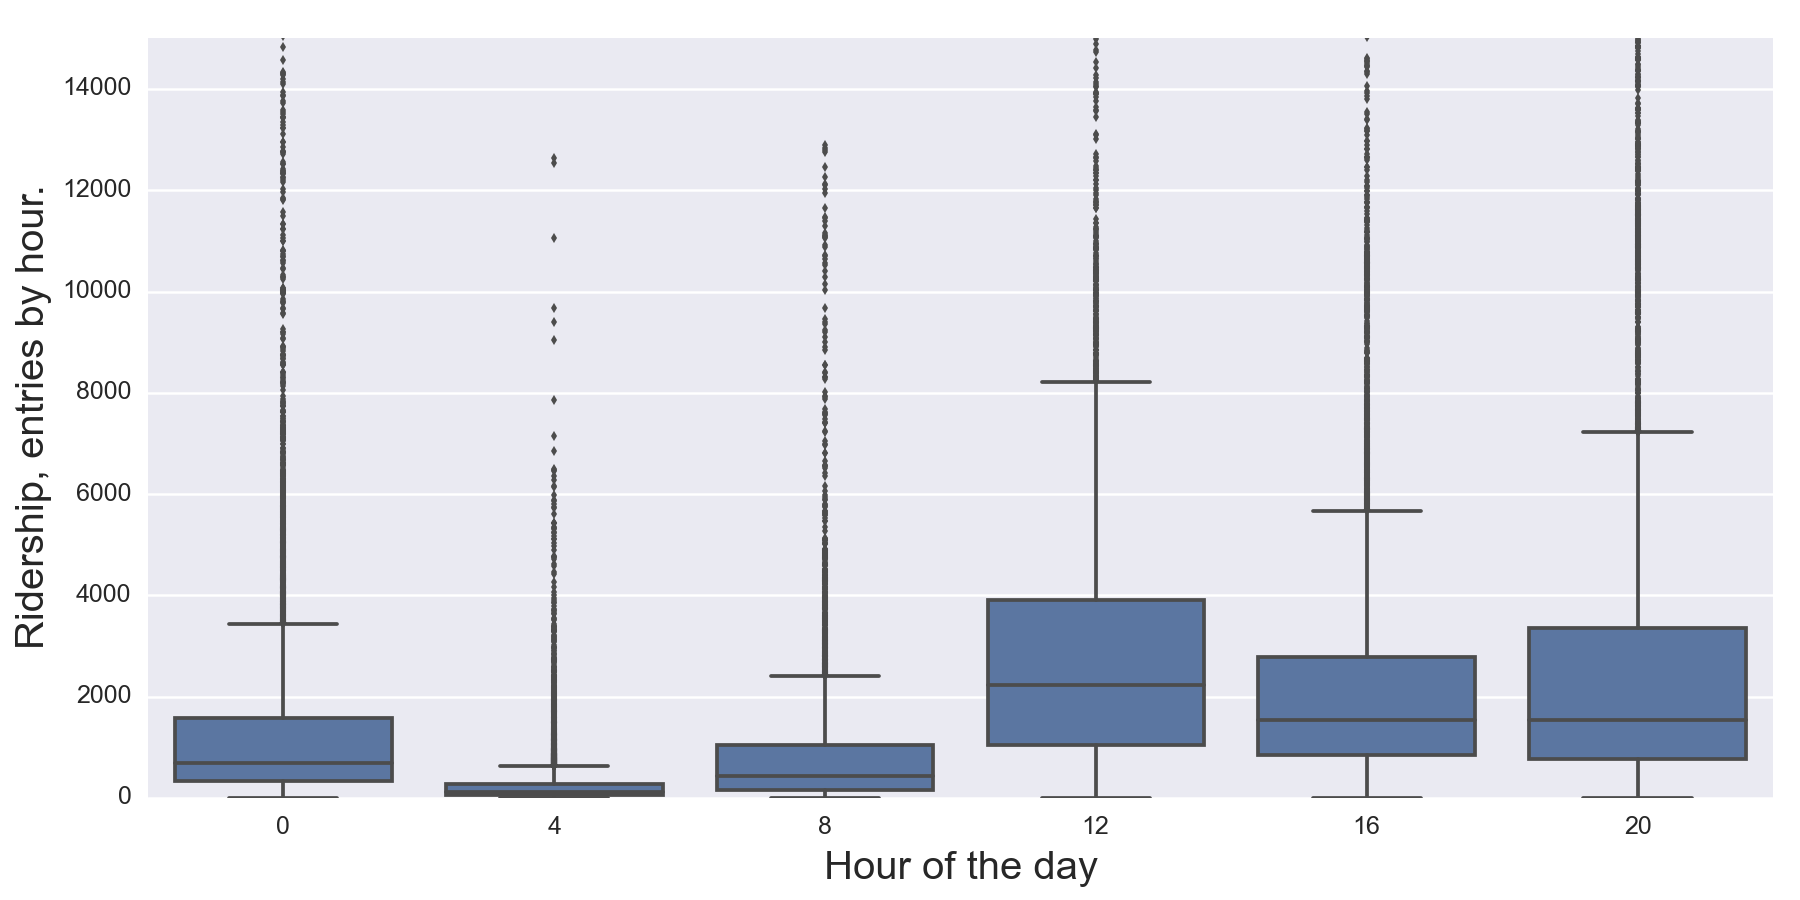
\includegraphics{hour_rider.png}}
\caption{Ridership vs hour of the day.}{\small 
Instead of just constructing a scatter plot, we decided to use another descriptive
statistic method to study the relation, if any, between ridership and hour of
the day. We used boxplots to visualize the distribution of ridership for each
hour of the day. In this way we can see that the medians do not follow a
linear relation with the hour of the day, and that there is a huge spread
of possible ridership values for each hour.
}\label{section2:figure31}\end{figure}
\begin{itemize}
\item {} 
\emph{weekday}: numerical (and categorical) variable indicating if the day
when the ridership measurement was done was either a weekday (1) or weekend
day (0). {\hyperref[section2:figure32]{\emph{Figure 3.2}}}
shows the relation of the ridership with kind of day.

\end{itemize}
\begin{figure}[htbp]
\centering
\capstart

\scalebox{0.800000}{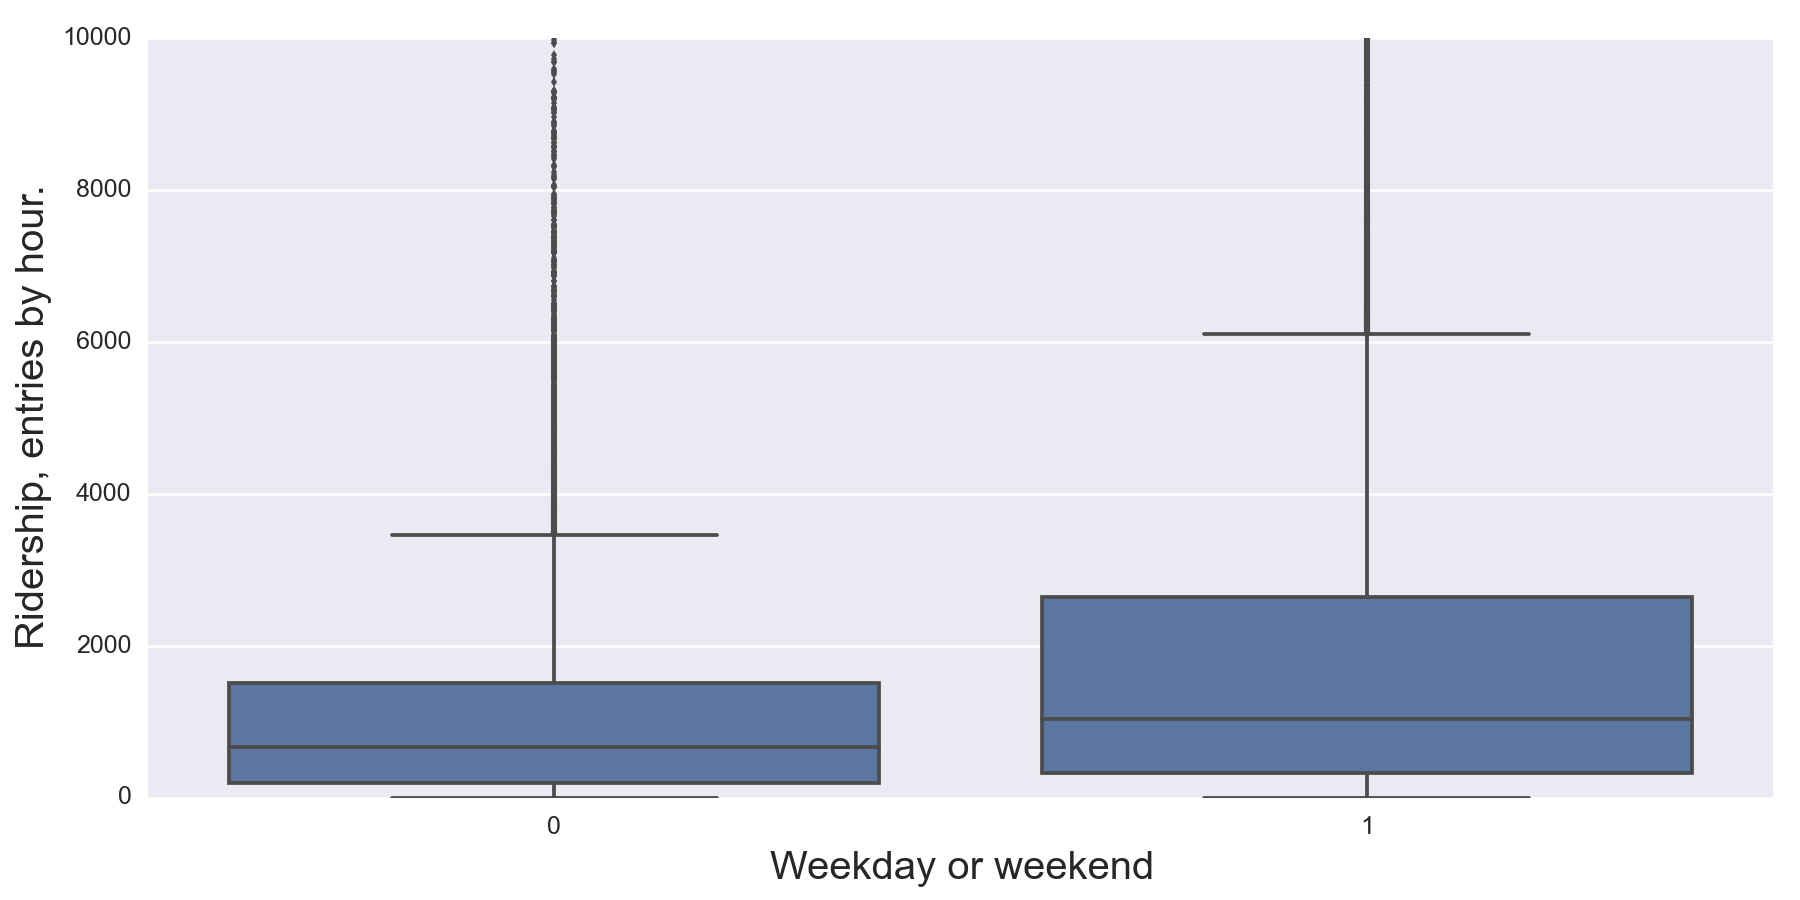
\includegraphics{weekday_rider.png}}
\caption{Ridership vs weekday/weekend-day.}{\small 
This plot show the ridership distribution as boxplots for work days (Monday to
Friday) and weekend days (Saturdays and Sundays). It is clear that even
when the spread in entries per hour is still big a linear correlation can
be used.
}\label{section2:figure32}\end{figure}
\begin{itemize}
\item {} 
\emph{rain}: daily precipitation condition for a turnstile location (0 for a clear
day, 1 for rainy). Even when is a categorical variable, it is also numerical,
and it is used as the final predictor feature for our liner model.
{\hyperref[section2:figure33]{\emph{Figure 3.3}}} shows the relation of the ridership values with
precipitation conditions.

\end{itemize}
\begin{figure}[htbp]
\centering
\capstart

\scalebox{0.800000}{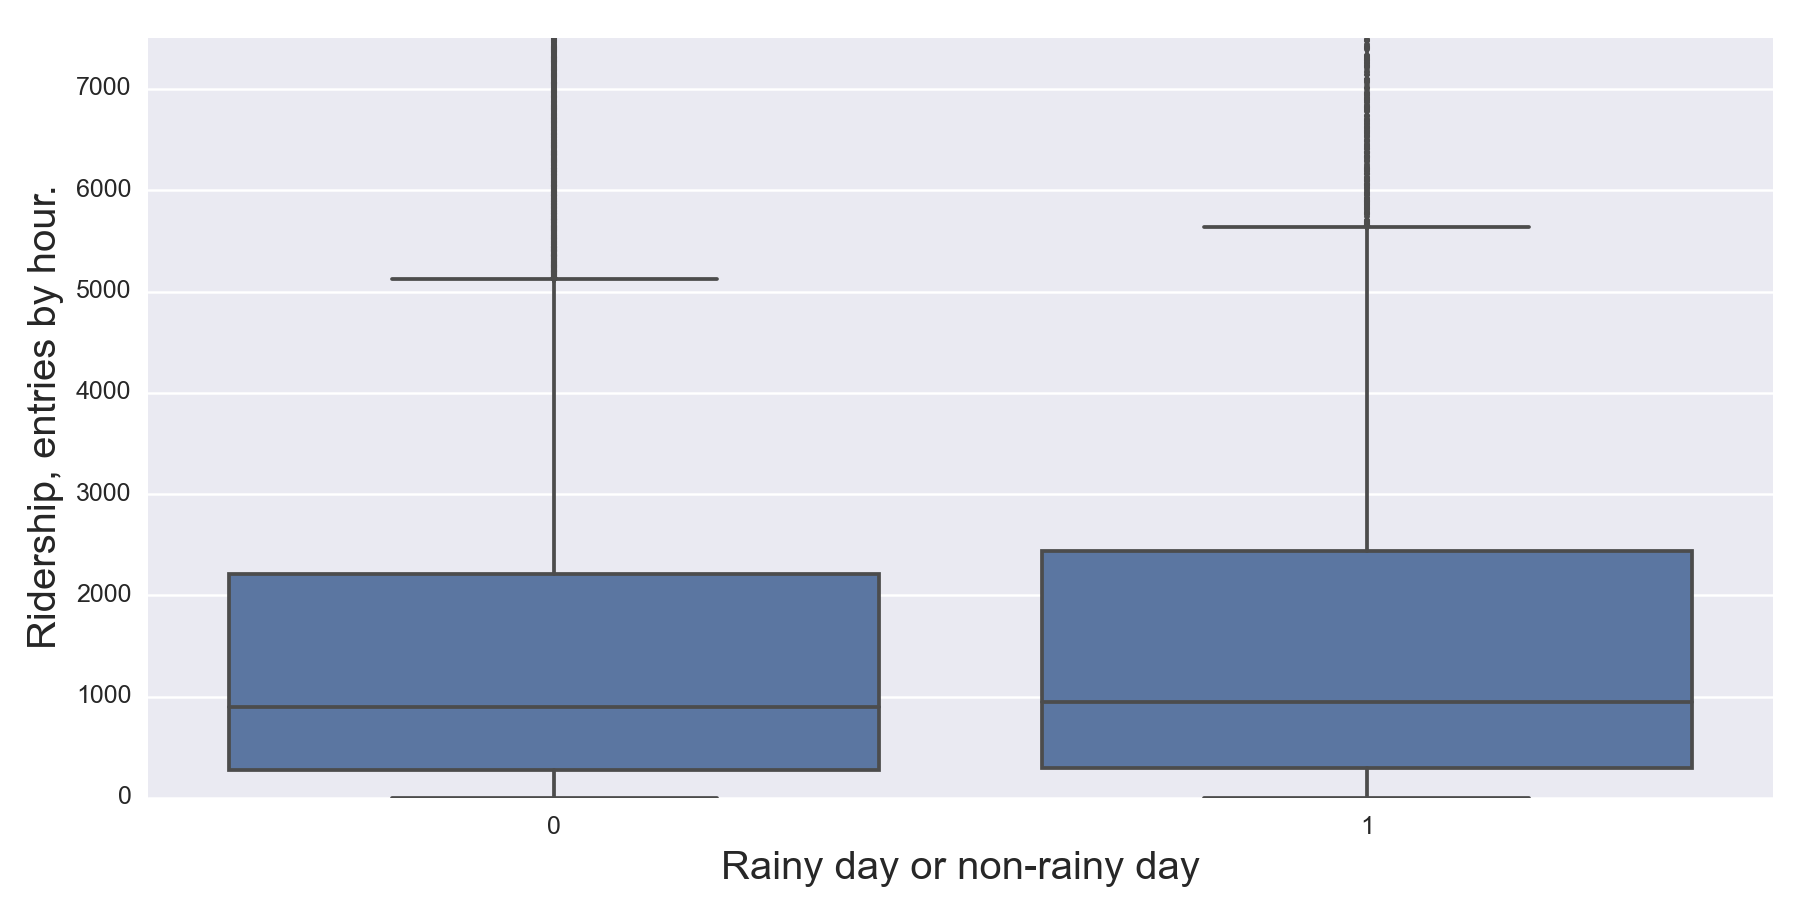
\includegraphics{rain_rider.png}}
\caption{Ridership vs rainy conditions.}{\small 
With the use of boxplots again, we can see in this figure that a really mild
linear relation exist for the relation between daily precipitation conditions
and ridership. (Which as was shown in the previous section is not significant)
}\label{section2:figure33}\end{figure}

The features were selected based partially on intuition and partially by exploratory
analysis.

First, it was clear that the behavior, for each individual turnstile, was mainly
a function of the hour of the day and the day of the week, as is shown in
{\hyperref[section2:figure34]{\emph{Figure 3.4}}}: there is a clear periodicity in the ridership
behavior for each day, depending on the time of the day, and also a dependence
on the day of the week. However the relation is clearly non-linear. We kept the
\emph{hour} as a predictor because is an important predictor, an in a very rough way
one can see that ridership is lower in the beginning of the day while reaching
a pick on the evenings.
\begin{figure}[htbp]
\centering
\capstart

\scalebox{1.000000}{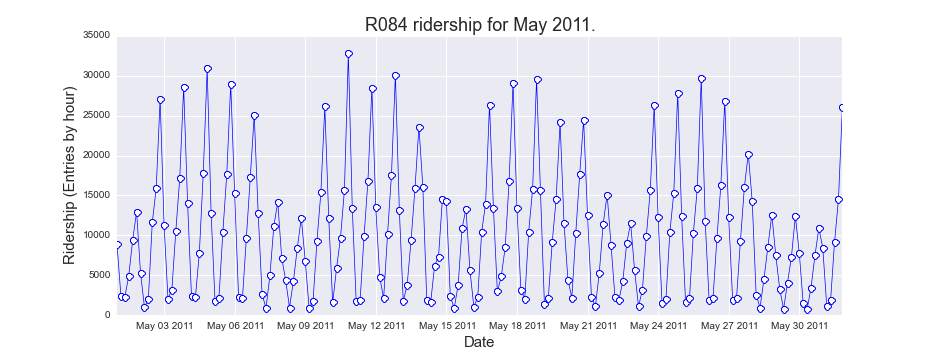
\includegraphics{r084_may.png}}
\caption{Ridership vs date for turnstile R084.}{\small 
The figure clearly shows a periodic behavior for the ridership behavior for
a particular turnstile, which is a function mainly of the hour of the day and
day of the week. Ridership picks are usually seen at 20 hours, while weekends
and holidays (May 30th) being less busy than weekdays.
}\label{section2:figure34}\end{figure}

However, we decided to use \emph{weekday} instead of \emph{day\_week} (the second being the
day of the week, i.e, a number between 0 and 6, where 0 i Monday and 6 Sunday),
because the major change on ridership behavior is seen between work days and
off days (weekends), and \emph{weekday} can be better modeled by a linear model than
\emph{day\_week} (as it can be checked on {\hyperref[section2:figure35]{\emph{Figure 3.5}}})
\begin{figure}[htbp]
\centering
\capstart

\scalebox{0.800000}{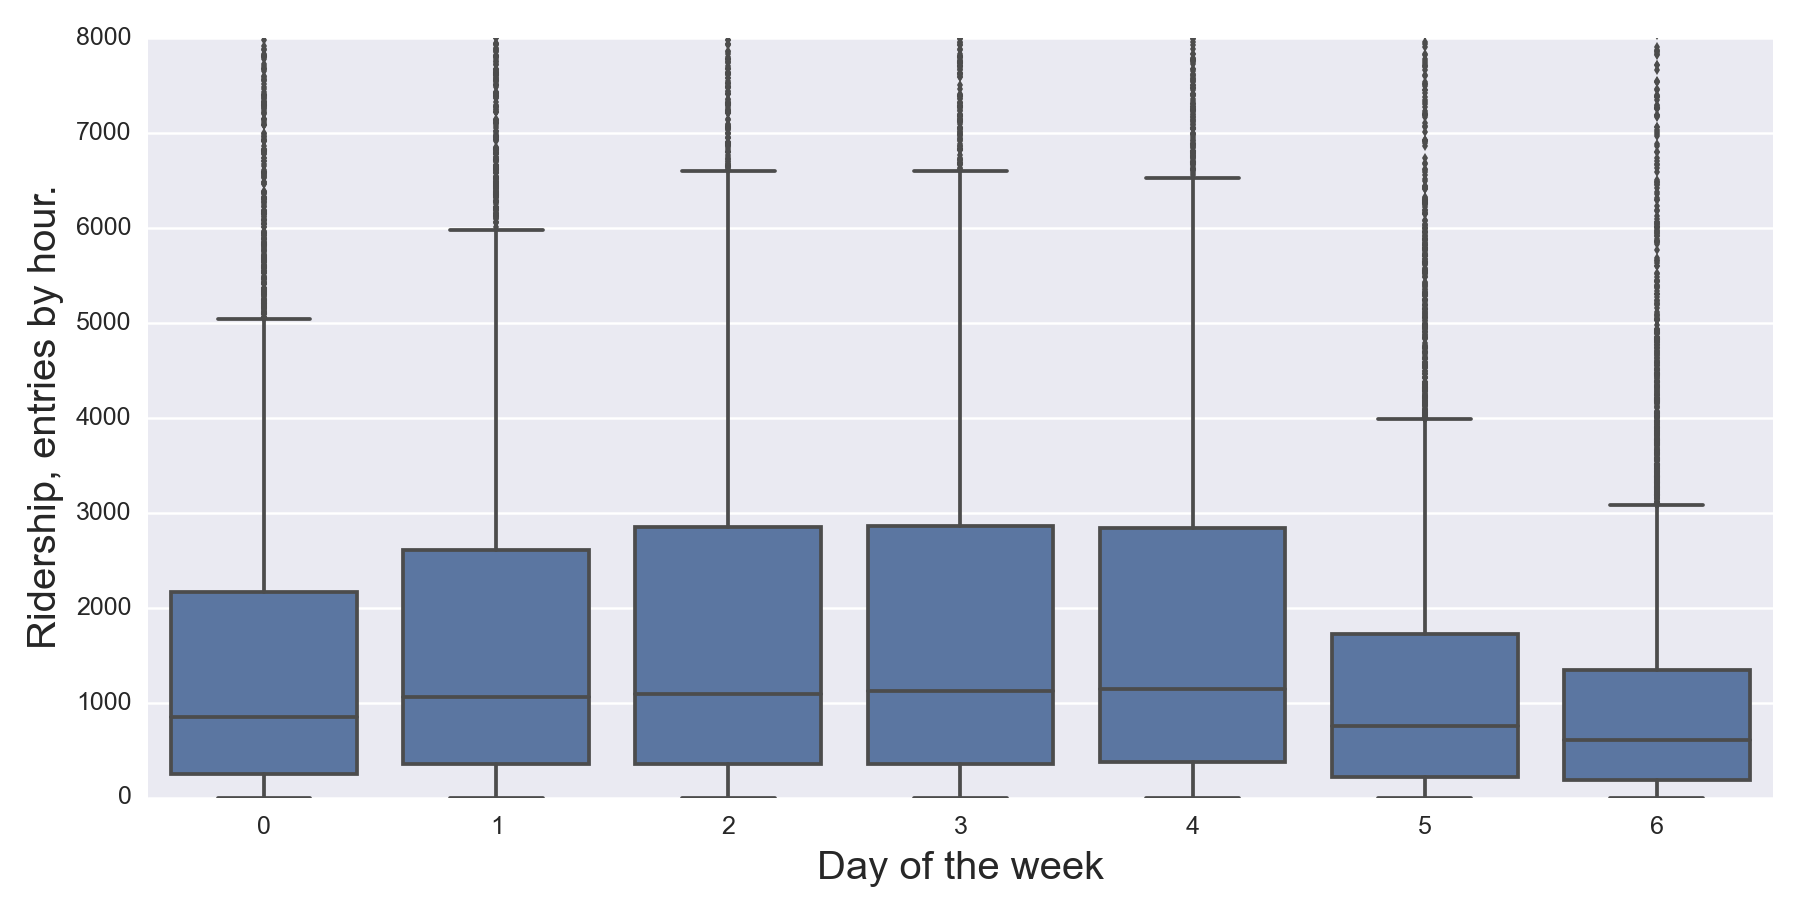
\includegraphics{day_rider.png}}
\caption{Ridership vs day of the week.}{\small 
This plot show the ridership distribution as boxplots for the 7 days of the
week (0 is Monday, 6 is Sunday). We can see that even when a relation
exist between day of the week and ridership, this relation doesn't look
linear, and thus we decided to use \emph{weekday} instead.
}\label{section2:figure35}\end{figure}


\section{Results: coefficients and R Squared}
\label{section2:results-coefficients-and-r-squared}
The coefficients found with the gradient descent and OLS algorithms were the
same in both cases, which was expected for a successful execution of the
gradient descent algorithm. The selected features were enough to obtain a
\(R^2 = 0.481\). More in depth details of the result can be seen in
{\hyperref[section2:table31]{\emph{Table 3.1}}}. Also, thanks to the statsmodels OLS implementation
we can report some of the coefficients obtained from the linear model fit,
using the predictor variables \emph{hour}, \emph{weekday}, \emph{rain} and dummies from \emph{UNIT}
({\hyperref[section2:multreg-mod]{\emph{Eq. 3.1}}}), and their statistical significances
({\hyperref[section2:table32]{\emph{Table 3.2}}}).

At {\hyperref[section2:figure36]{\emph{figure 3.6}}} we present some residuals analysis plots, in order
to provide later a more accurate interpretation of these results.
\phantomsection\label{section2:table31}

\begin{threeparttable}
\capstart\caption{OLS Regression Results}

\begin{tabulary}{\linewidth}{|L|L|}
\hline
\textsf{\relax 
OLS Regression Results
} & \textsf{\relax }\\
\hline
Dep. Variable:        ENTRIESn\_hourly
 & 
R-squared:                       0.481
\\

Model:                            OLS
 & 
Adj. R-squared:                  0.478
\\

Method:                 Least Squares
 & 
F-statistic:                     163.1
\\

Date:                Wed, 07 Jan 2015
 & 
Prob (F-statistic):               0.00
\\

Time:                        14:12:52
 & 
Log-Likelihood:            -3.8397e+05
\\

No. Observations:               42267
 & 
AIC:                         7.684e+05
\\

Df Residuals:                   42027
 & 
BIC:                         7.705e+05
\\

Df Model:                         239
 & \\

Covariance Type:            nonrobust
 & \\
\hline\end{tabulary}

\end{threeparttable}

\phantomsection\label{section2:table32}

\begin{threeparttable}
\capstart\caption{Linear regression coefficients}

\begin{tabulary}{\linewidth}{|L|L|L|L|L|L|}
\hline
\textsf{\relax 
Predictor
} & \textsf{\relax 
coef
} & \textsf{\relax 
std err
} & \textsf{\relax 
t
} & \textsf{\relax 
P\textgreater{}\textbar{}t\textbar{}
} & \textsf{\relax 
{[}95\% Conf. Int.{]}
}\\
\hline
\textbf{Intercept}
 & 
-1750.5171
 & 
166.661
 & 
-10.503
 & 
0.000
 & 
-2077.175 -1423.859
\\

C(UNIT){[}T.R004{]}
 & 
334.1581
 & 
231.108
 & 
1.446
 & 
0.148
 & 
-118.819   787.135
\\

C(UNIT){[}T.R005{]}
 & 
335.0522
 & 
232.095
 & 
1.444
 & 
0.149
 & 
-119.859   789.963
\\

C(UNIT){[}T.R006{]}
 & 
451.3319
 & 
229.532
 & 
1.966
 & 
0.049
 & 
1.445   901.218
\\

C(UNIT){[}T.R007{]}
 & 
164.5844
 & 
232.767
 & 
0.707
 & 
0.480
 & 
-291.644   620.812
\\

...
 & 
...
 & 
...
 & 
...
 & 
...
 & 
...       ...
\\

\textbf{hour}
 & 
124.0989
 & 
1.500
 & 
82.741
 & 
0.000
 & 
121.159   127.039
\\

\textbf{weekday}
 & 
980.9091
 & 
23.243
 & 
42.203
 & 
0.000
 & 
935.353  1026.465
\\

\textbf{rain}
 & 
36.3145
 & 
25.167
 & 
1.443
 & 
0.149
 & 
-13.013    85.642
\\
\hline\end{tabulary}

\end{threeparttable}

\begin{figure}[htbp]
\centering
\capstart

\scalebox{1.000000}{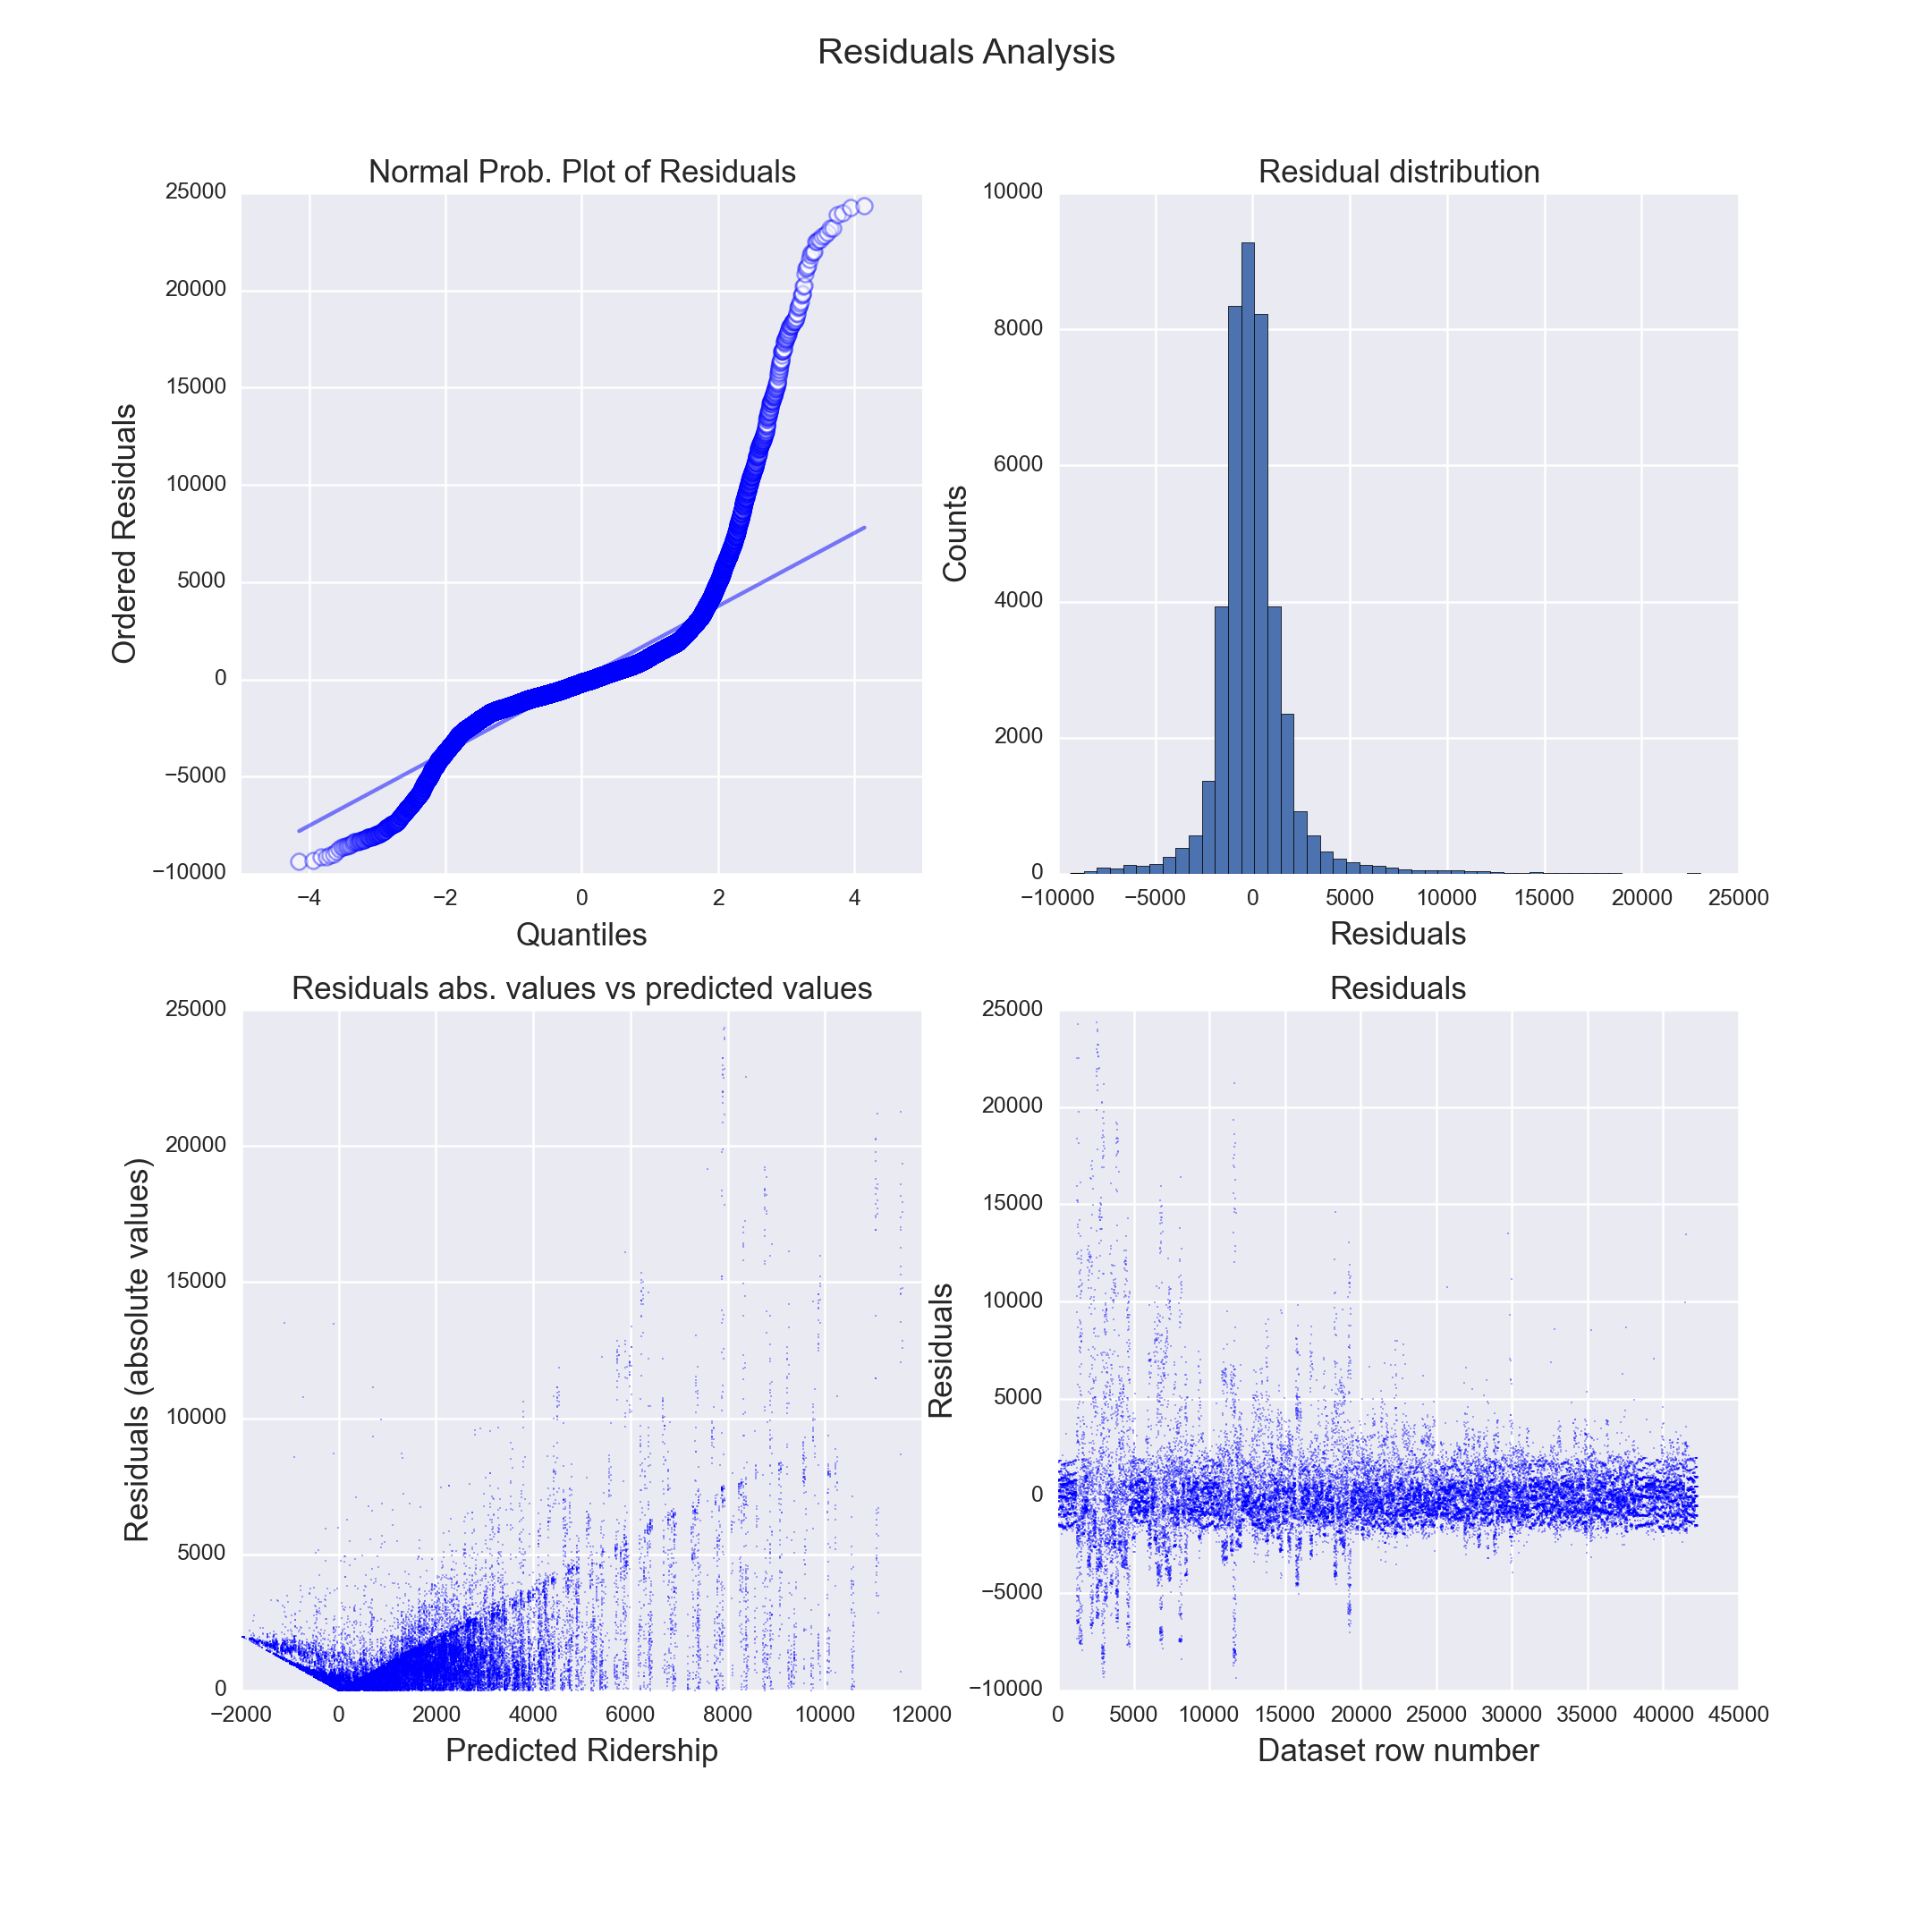
\includegraphics{residuals_an.png}}
\caption{Residuals analysis plots for the linear regression model (improved dataset).}{\small 
\emph{Top left:} normal probability plot of the residuals and \emph{top right:} residuals
distribution. It is clear that residuals do not adjust well to a simple normal
probability distribution. \emph{Bottom left} shows the residuals versus the
predicted quantities, and \emph{bottom right} just shows the residuals distribution
around 0.
}\label{section2:figure36}\end{figure}


\section{Interpretation and limits}
\label{section2:interpretation-and-limits}\begin{figure}[htbp]
\centering
\capstart

\scalebox{0.900000}{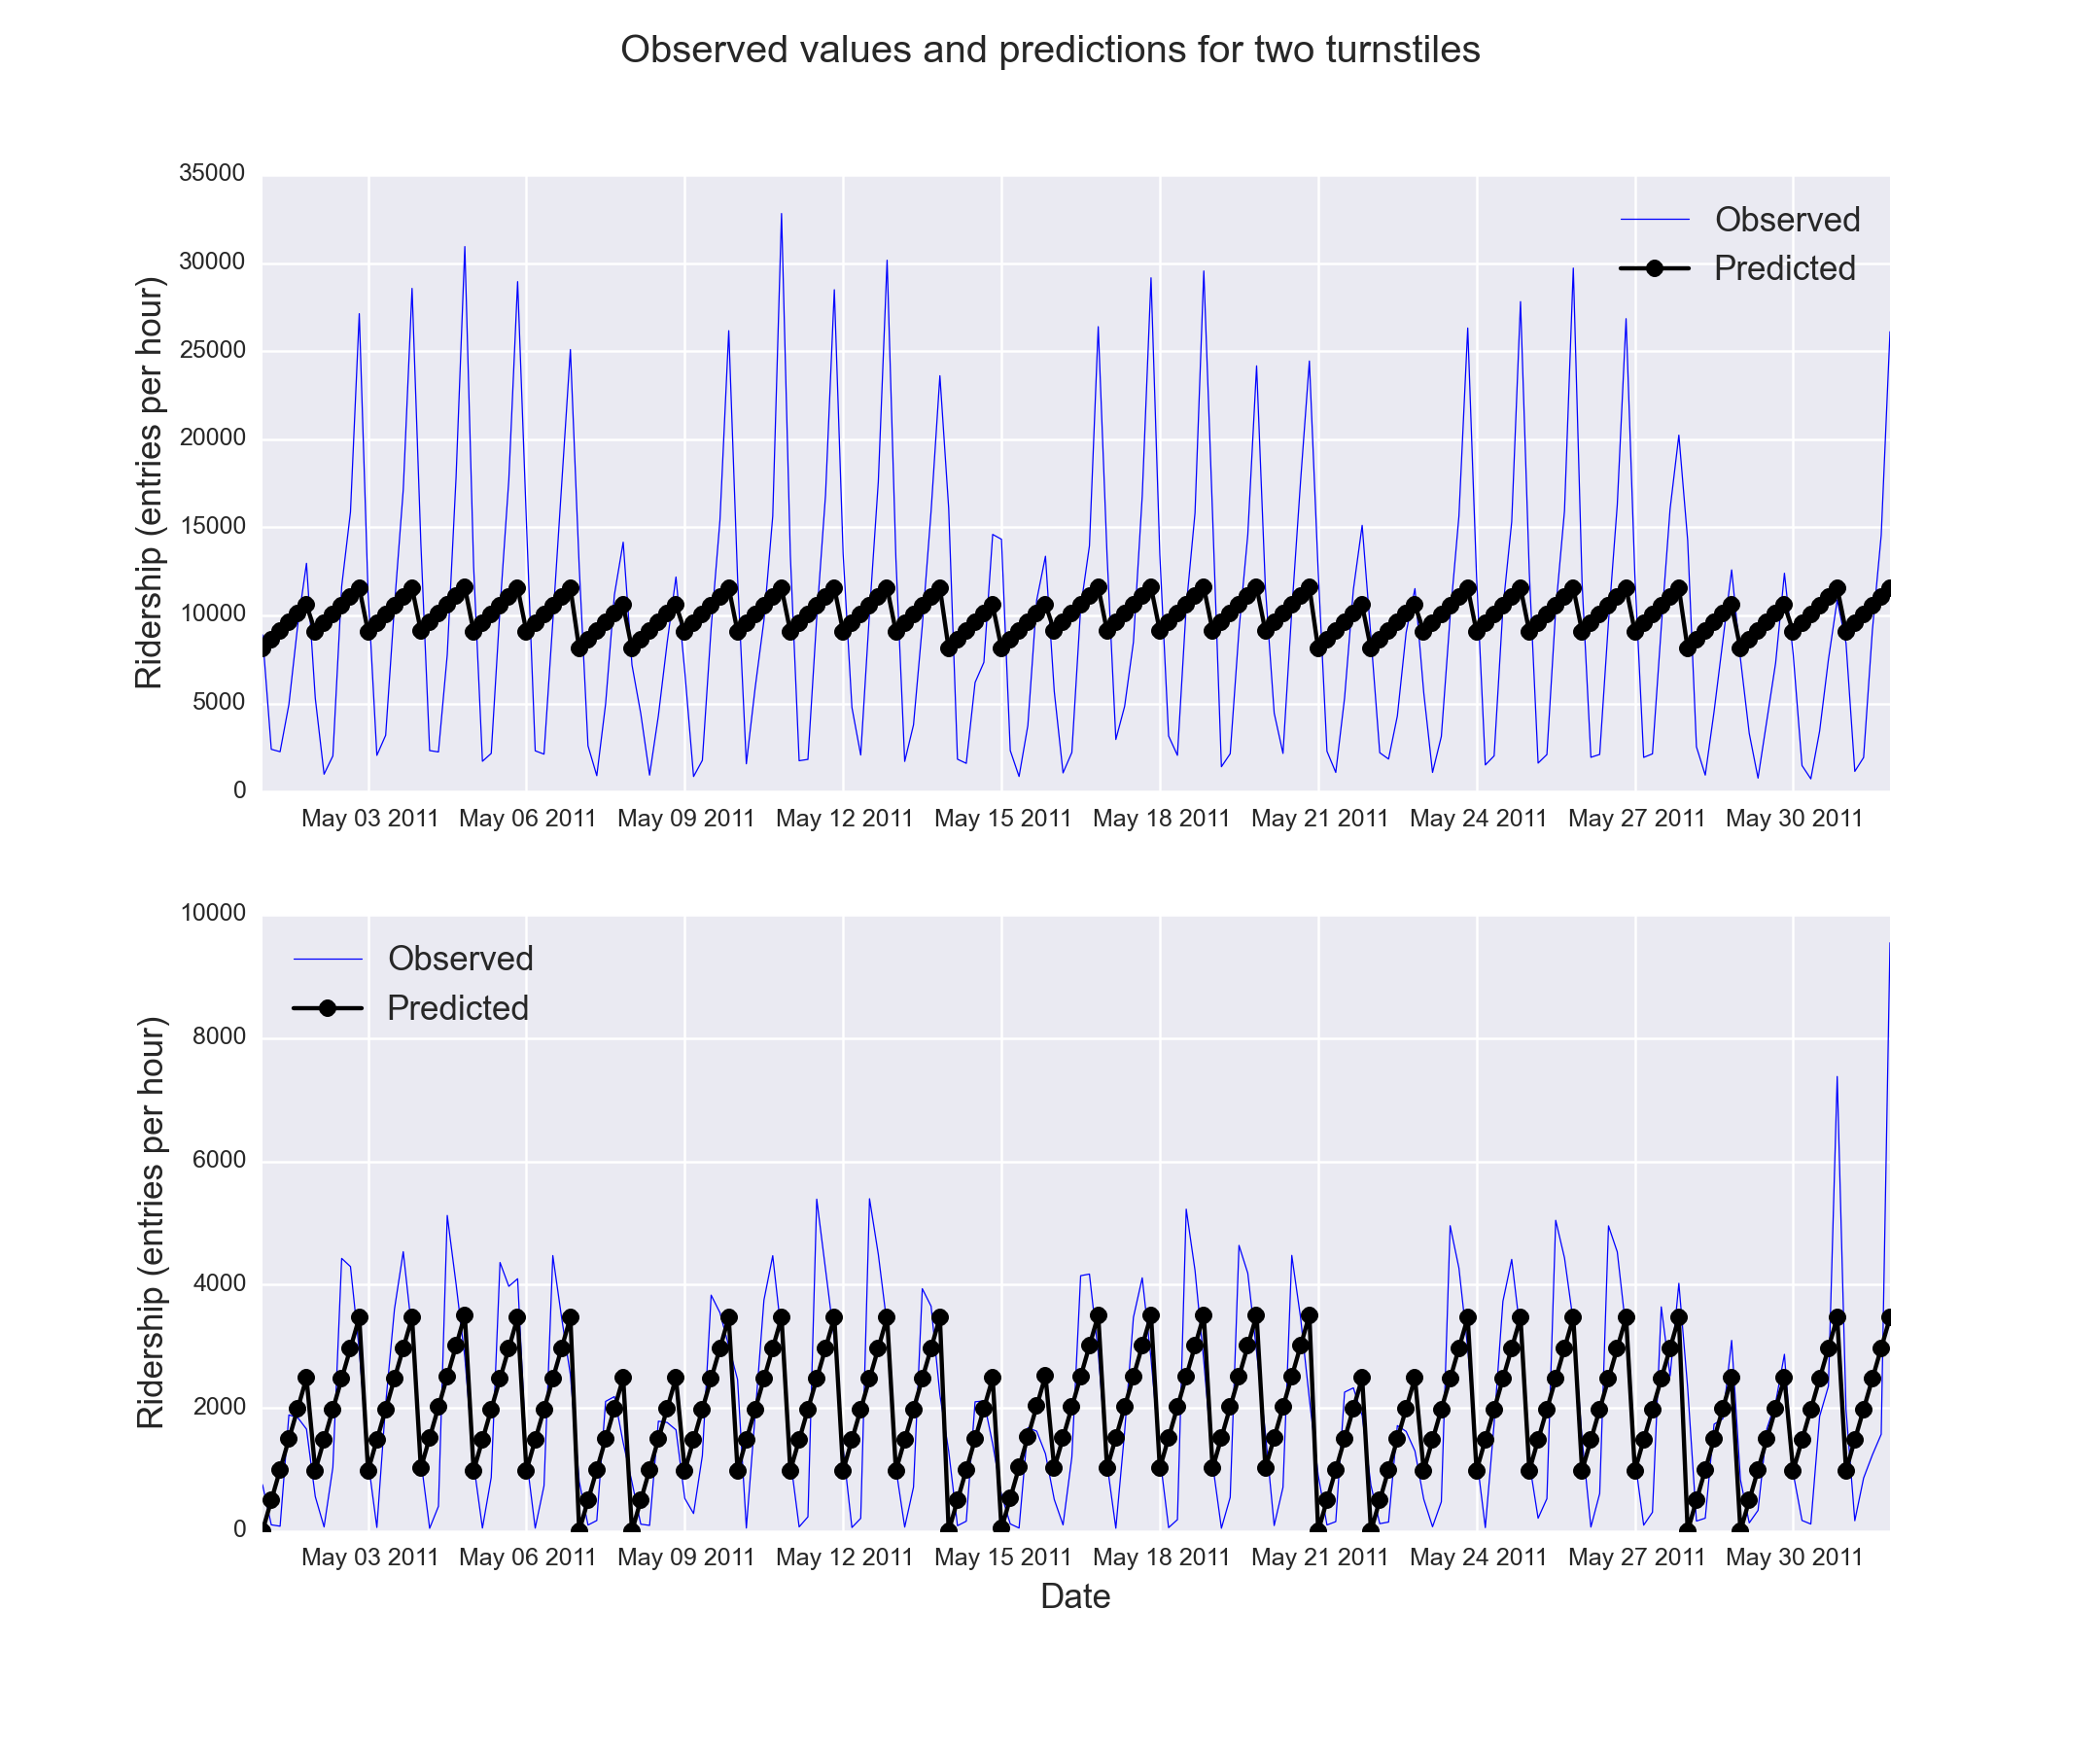
\includegraphics{turns_pred.png}}
\caption{The observed ridership values for two different turnstiles in the month of May,
over-plotted with the predicted ridership for both cases.}{\small 
The turnstiles used were R084 and R172, one at downtown and the other at the
periphery. The predicted values come from the linear regression model applied
in previous section.
}\label{section2:figure37}\end{figure}

A successful multiple regression model should comply with several assumptions,
which can be checked by analysing the residuals.
\begin{enumerate}
\item {} 
\end{enumerate}


\chapter{Visualization}
\label{section3:visualization}\label{section3::doc}

\section{Ridership distribution with weather}
\label{section3:ridership-distribution-with-weather}

\section{Supporting visualizations}
\label{section3:supporting-visualizations}

\chapter{Conclusion}
\label{section4::doc}\label{section4:conclusion}

\chapter{Reflection}
\label{section5::doc}\label{section5:reflection}

\section{Shortcomings and limitations}
\label{section5:shortcomings-and-limitations}

\section{Insights}
\label{section5:insights}
\begin{thebibliography}{os4}
\bibitem[os4]{os4}{\phantomsection\label{section1:os4} 
Diez, Barr, Cetinkaya-Rundel. Open Intro Statistics. 2nd Edition.
openintro.org
}
\end{thebibliography}



\renewcommand{\indexname}{Index}
\printindex
\end{document}
